\section{Introduction}
\begin{figure*}[h]
	\centering
	% \printinunitsof{in}\prntlen{\textwidth}
	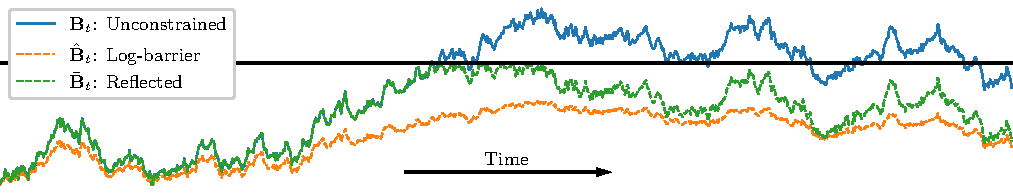
\includegraphics[width=\textwidth]{images/constrained_diffusion/reflected_vs_brownian_1d.pdf}
	\caption{The behaviour of different types of noising processes considered in this chapter defined on the unit interval. \(\mathbf{B}_t\): Euclidean (unconstrained) Brownian motion.
		\(\hat{\mathbf{B}}_t\): Log barrier forward noising process. \(\bar{\mathbf{B}}_t\): Reflected Brownian motion.
		All sampled with the same initial point and driving noise.
		Black line indicates the boundary.
	}
	\label{fig:reflected_vs_brownian}
\end{figure*}

\lettrine{A}{key assumption} made in the previous chapter when generalising score-based models to Riemannian manifolds is that the stochastic processes considered as noising processes are defined \emph{for all times}.
While this holds for a large class of stochastic processes and manifolds, it is not the case for most manifolds with boundary defined via a set of inequality constraints.
The key assumption that allowed this to hold was that the manifolds were \emphhypermargin{geodesically complete}{def:geodesically_complete}.

For instance, in the case of the \emphmarginnote{hypercube}, \(\del{-1,1}^d\) equipped with the Euclidean metric, the Riemannian Brownian motion coincides with the Euclidean \(d\)-dimensional Brownian motion \((\v{B}_t)_{t \in \cbr{0,T}}\) as long as \(\v{B}_t \in \del{-1,1}\).
However, with probability one \((\v{B}_t)_{t \geq 0}\) escapes from \(\del{-1,1}^d\), meaning that the Riemannian Brownian motion is not defined for times after this escape, and the framework of the \cref{cpt:riemannian_score_based_models} does not apply.

Such \emphmarginnote{constrained manifolds} comprise a wide variety of settings---including polytopes and convex sets of Euclidean spaces---and are studied across a wide range of disciplines, ranging from computational statistics \parencite{Morris2002}, robotics \parencite{han2006inverse} quantum physics \parencite{lukens2020practical}, and computational biology \parencite{Thiele2013}.
Deriving principled diffusion models that are able to operate directly on these manifolds is thus of significant practical importance.
This enables generative modelling in data-scarce and safety-critical settings in which constraints on the modelled domain may reduce the number of degrees of freedom or prevent unwanted behaviour.

As sampling problems on such manifolds are important, a flurry of Markov chain based methods have been developed to sample from unnormalised densities \parencite{kook2022sampling,heirendt2019creation}.
Successful algorithms include the \emphmarginnote{reflected Brownian motion} \parencite{williams1987Reflected,petit1997Time,shkolnikov2013Timereversal}, \emphmarginnote[\baselineskip]{log-barrier methods} \parencite{Kannan2009,lee2017Geodesic,noble2022Barrier,kook2022sampling,gatmiry2022convergence,lee2018convergence} and hit-and-run approaches in the case of polytopes \parencite{Smith1984,Lovasz2006}.

In this chapter, we study the generative modelling counterparts of these algorithms through the lens of diffusion models.
Among existing methods for statistical sampling on constrained manifolds, the geodesic Brownian motion \parencite{lee2017Geodesic} and the reflected Brownian motion \parencite{williams1987Reflected} are continuous stochastic processes, and thus well suited for extending the continuous Riemannian diffusion framework developed in the previous chapter.
In particular, we introduce two principled diffusion models for generative modelling on constrained domains based on \begin{enumerate}[label=(\roman*)] \item the geodesic Brownian motion, leveraging tools from the log-barrier methods, discussed in \cref{sec:bsgm}, and \item the reflected Brownian motion, discussed in \cref{sec:rbm}. \end{enumerate}
In both cases, we show how one can extend the ideas of time-reversal and score matching to these settings.
We demonstrate the practical utility of these methods on a range of tasks defined on convex polytopes and the space of symmetric positive definite matrices, including the constrained conformational modelling of proteins and robotic arms.
While both models extend classical diffusion models to inequality-constrained settings, they exhibit very different behaviours.
We discuss their practical differences in \cref{sec:diff_methods}.

% \section{Background}
% \paragraph{Riemannian manifolds.}
% A Riemannian manifold is a tuple \((\c{M}, {g})\) with \(\c{M}\) a smooth manifold and \({g}\) a metric which defines an inner product on tangent spaces.
% The metric \({g}\) induces key quantities on the manifold, such as an exponential map \(\exp_x: \mathrm{T}_x \c{M} \rightarrow \c{M}\), defining the notion of following straight lines on manifolds, a gradient operator \(\nabla\), the (Riemannian) gradient \(\nabla\) is defined s.t.
% for any smooth \(f\in \mathrm{C}^\infty(\c{M})\), \(x \in \c{M}, v \in \mathrm{T}_x\c{M}\), \({g}(x)(f(x), v) = \mathrm{d} f(x) (v)\), and divergence operator \(\mathrm{div}\), the Riemannian divergence acts vector fields and can be defined using the volume form of \(\c{M}\).

% It also induces the Laplace-Beltrami operator \(\Delta\) and consequently a Brownian motion with density (w.r.t.
% the volume form \footnote{We assume that \(\c{M}\) is orientable and therefore that a volume form exists })whose density is given by the heat equation \({\partial_t } p_t = \Delta p_t\).
% We refer the reader to \cref{sec:riemannain_intro} for a brief introduction to differential geometry, to \textcite{lee2013smooth} for a thorough treatment and to \textcite{hsu2002stochastic} for details on stochastic analysis on manifolds.
\begin{figure}
	\centering
	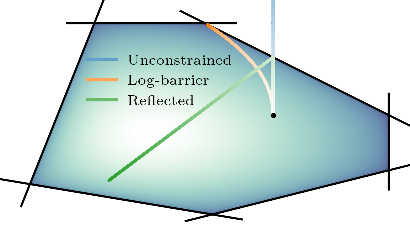
\includegraphics[width=0.7\textwidth]{images/constrained_diffusion/polytope2.pdf}
	\caption{
	A convex polytope defined by six constraints \(\{f_i\}_{i \in \c{I}}\), along with the log barrier potential, and geodesics under the log-barrier metric and under the Euclidean metric with and without  reflection at the boundary.
	}
	\label{fig:polytope}
\end{figure}
\subsection{Technical setting}
\label{sec:constrained_diffusion_models}


In this chapter, we are concerned with what we shall term \emph{constrained} manifolds.
More precisely, given a Riemannian manifold \((\c{N}, {h})\), we consider a family of real functions \(\{f_i: \c{N} \to \R\}_{i \in \mathcal{I}}\) indexed by \(\mathcal{I}\).
We then define \begin{equation} \label{eq:constrained} \c{M} = \cbr{x \in \c{N} \; : \; f_i(x) < 0 , \ i \in \mathcal{I}},
\end{equation}
and derive models such that their densities are constrained to be in the set \(\c{M}\).

In this scenario, \(\{f_i\}_{i \in \mathcal{I}}\) are interpreted as a set of constraints on \(\c{N}\).
For example, choosing \(\c{N} = \R^d\) and affine constraints \(f_i(x) = \langle a_i, x\rangle - b_i\), \(x\in \R^d\), we get that \(\c{M}\) is an open polytope as illustrated in \cref{fig:polytope}.
This setting naturally appears in many areas of engineering, biology, and physics \parencite{boyd2004convex, han2006inverse, lukens2020practical}.

This setting is very similar to that of a \emphhypermargin{manifold with boundary}{def:manifold_with_boundary}. 
If the interior of the constraints form an open set on the manifold then we can consider this as exactly as a manifold with boundary.
We consider the constraints in the way set out as it allows us to consider a slightly larger setting, and is computationally a little easier to deal with.
In light of this we term the set
\[\partial \c{M} = \cbrcolon{x \in \c{M}}{f_i(x) = 0 \text{ for any } i \in I \text{ and } f_i(x) \not\geq 0 \text{ for any } i\in I}\]
the boundary, although this slightly abuses the terminology of a manifold with boundary.

While the two methods we introduced in this chapter can be applied to the general framework, in our applications, we focus on two specific settings: \begin{enumerate}[label=(\alph*)] \item \emphmarginnote{polytopes}---\(\c{N} = \R^d\) with linear boundaries forming a convex set, \item \emphmarginnote{symmetric positive definite matrices} (SPD) under maximum trace conditions---\(\c{N}=\mathcal{S}_{++}^{d}\), a quadratic boundary on the elements of the matrix.
\end{enumerate}

\section{Log-barrier diffusion models}
% \FloatBarrier
\label{sec:bsgm}

\begin{figure*}[h]
	\begin{minipage}[b]{0.49\textwidth}
		\centering
		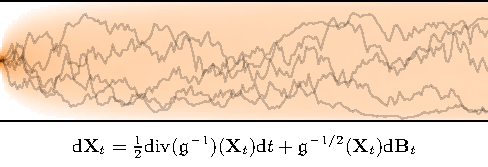
\includegraphics{images/constrained_diffusion/hessian_density.pdf}
		\caption{Convergence of the barrier Langevin dynamics on the unit interval to the uniform distribution.}
		\label{fig:density}
	\end{minipage}
	\hfill
	\begin{minipage}[b]{0.49\textwidth}
		\centering
		\begin{tikzpicture}
			\tikzset{
				punkt/.style={
						rectangle,
						rounded corners,
						draw=black, very thick,
						text width=9em,
						minimum height=2em,
						text centered},
				pil/.style={
						<->,
						thick,
						shorten <=2pt,
						shorten >=2pt,}
			}
			\node[punkt, text width=6em] (a) at (0,0) {\((\mathcal{N}, h)\)};%
			\node[punkt, text width=6em, right=5em of a] (b) {\((\mathcal{M}, \nabla^2 \phi)\)}
			edge[pil] (a.east);
			\node[draw, above=1em of a] (e) {Original space};
			\node[draw, above=1em of b] (f) {Constrained space};
		\end{tikzpicture}
		\vspace{2.7em}
		\caption{
			Illustrative diagram of the barrier method and the change of metric.
		}
	\end{minipage}
\end{figure*}

First we consider a method based on \emphmarginnote{barrier methods}.
Barrier methods work by constructing a smooth potential \(\phi: \c{M} \rightarrow \R\) such that it blows up on the boundary of a desired set, see \textcite{nesterov2018lectures}.
Such potentials are at the basis of interior methods in optimisation \parencite{boyd2004convex}.

For a single boundary, \(\partial \c{M}\) to define a barrier function it is sufficient to be able to measure the distance to the boundary, \[d(x, \partial \c{M}) = \min_{y\in \partial \c{M}} d(x, y),\] and a monotone decreasing function \(\phi: \R^+ \to \R\) such that \(\lim_{z \rightarrow 0} \phi(z) = \infty\) (plus some technical conditions, see \cite{nesterov1994interior}).
We can then define the barrier function as \(\phi(d(x, \partial{M}))\).

In the setting with multiple constraints we can define the barrier as 
\[\phi(\min_{i\in I} d(x, f_i)), \]
where \(f_i\) is the set defined by \(f_i(y) = 0, y\in \c{N}\).
We can also define the barrier as 
\[\sum_{i\in I} \phi(d(x, f_i)).\]
If \(\phi\) is smooth this guarantees the barrier function to be smooth, unlike the first construction.

Of the functions we can choose for \(\phi\), \(\phi(x) = -\log(x)\), is the most common, and methods based off this are known as \emphmarginnote{log barrier methods} \cite{lee2017Geodesic}.

In general solving the minimum distance to the boundary of a set is a highly non-trivial optimisation problem.
Linear boundaries are one case which admits a simple closed form.
For a convex polytope \(\c{M}\) defined by the constraints \(\mathrm{A} x < b\), with \(\mathrm{A} \in \R^{m \times d}\) and \(b \in \R^m\), giving \(m\) constrains, the distance to \(i\)\textsuperscript{th} boundary is given by
\[d(x, f_i) = \innerprod{A_i}{x} - b_i.\]
The log barrier \(\phi: \ \c{M} \to \R_+\) is therefore given by \begin{equation} \label{eq:log_barrier_polytope} { \phi(x) = - \sum_{i=1}^m \log(\langle \mathrm{A}_i, x\rangle-b_i),
	}
\end{equation}
assuming that \(\| \mathrm{A}_i \| =1\).

The core idea of barrier methods is to `warp the geometry' of the constrained space, stretching it as the boundary is approached so it is never hit.
This bypasses the need to explicitly deal with the boundary.

\subsection{Hessian metrics}

Let us assume that \(\c{N} = \R^d\), that the constraints \(\del{f_i}_{i\in\c{I}}\) form a convex compact set, and that we have a barrier function \(\phi\) which is strictly convex and smooth on \(\c{M}\), the interior of the constraints.

Assuming this, the Hessian \(\nabla^2 \phi\) is positive definite and thus defines a valid Riemannian metric on \(\c{M}\).
We endow \(\c{M}\) with \(g = \nabla^2 \phi\) as a Riemannian metric, making it into a \emphmarginnote{Hessian manifold} \cite{shima1997geometry}.
It can be proved that for such a metric the resulting exponential map is defined on the whole tangent space for all points and therefore the manifold \((\c{M}, \nabla^2 \phi)\) is a manifold \emph{without} boundary \cite{lee2017Geodesic}.

In the special case where the barrier is given by \cref{eq:log_barrier_polytope}, we get for any \(x \in \c{M}\) 
\[ {g}(x) = \mathrm{A}^\top S^{-2}(x) \mathrm{A} \text{ with } S(x) = \text{diag}(b_i - \langle \mathrm{A}_i, x \rangle)_i. \]
While developed and most commonly used in optimisation, barrier methods can also be used for sampling \parencite{lee2017Geodesic}.

\subsection{Forward noising process}
Let us consider a compact set of Euclidean space equipped with a Euclidean metric, and a Hessian non-Euclidean metric described above.

We consider the following Langevin dynamics, relative to the Euclidean metric, as a forward process \begin{equation} \label{eq:langevin_hessian_manifold} { \mathrm{d} \v{X}_t = \tfrac{1}{2} \mathrm{div}({g}^{-1})( \v{X}_t) \mathrm{d} t + {g}( \v{X}_t)^{-\frac{1}{2}} \mathrm{d} \v{B}_t, } \end{equation} where the divergence of the metric \(\dive g^{-1}\) is given by the \emphhyperref{generalisation of the divergence to tensor fields}{def:tensor_field_divergence}.
On Euclidean space this is given by the column-wise divergence of \(g^{-1}\).

Under mild assumptions on \(\c{M}\), \(\mathrm{div}({g}^{-1})\) and \({g}^{-1}\) we get that \(( \v{X}_t)_{t \geq 0}\) is well-defined and for any \(t \geq 0\), \( \v{X}_t \in \c{M}\).
In particular, for any \(t \geq 0\), \( \v{X}_t\) does not reach the boundary.

In addition, \(( \v{X}_t)_{t \geq 0}\) is irreducible as a Markov process.
Hence, assuming that \(\c{M}\) is compact, the uniform distribution on \(\c{M}\) is the unique invariant measure of the process \(( \v{X}_t)_{t \geq 0}\) and \(( \v{X}_t)_{t \geq 0}\) converges to the uniform distribution as \(t\to\infty\), giving us a tractable reference distribution for score-based modelling.
We refer the reader to \cref{sec:geod-brown-moti} for a proof of these results.

This stochastic process was first proposed by \textcite{lee2017Geodesic} in the context of efficient sampling from the uniform distribution over a polytope.
Under similar conditions, \( \v{X}_t\) admits a density \(p_t\) with respect to the Lebesgue measure, and we have that \(\partial_t p_t = \tfrac{1}{2} \mathrm{Tr}({g}^{-1} \nabla^2p_t)\).

\subsection{Time-reversal}
Assuming that \({g}^{-1}\) and its derivative are bounded on \(\c{M}\), the time-reversal of \cref{eq:langevin_hessian_manifold} is given by \cref{thm:fokker-plank_time_reversal_manifold}, in particular we have \begin{align} \mathrm{d} \v{X}_t^\vsla{} & = {\sbr{-\frac{1}{2} \mathrm{div}({g}^{-1}) + \mathrm{div}({g}^{-1}) { + {g}^{-1} \nabla \log p_{T-t}}(\v{X}_t^\vsla{}) }\mathrm{d} t + {g}(\v{X}_t^\vsla{})^{-\frac{1}{2}} \mathrm{d} \v{B}_t} \\  & = { \left[\frac{1}{2} \mathrm{div}( {g}^{-1}) + {g}^{-1} \nabla \log p_{T-t}\right](\v{X}_t^\vsla{}) \mathrm{d} t + {g}(\v{X}_t^\vsla{})^{-\frac{1}{2}} \mathrm{d} \v{B}_t.
                 }  \label{eq:reversal_langevin_hessian_manifold}
\end{align}
\(\v{X}_0^\vsla{}\) is initialised with the uniform distribution on \(\c{M}\) (which is close to the one of \( \v{X}_T\) for large \(T\)).

We refer to \cref{sec:score-netw-param} for details on the training and parameterisation of the score function.

\subsection{Sampling}
Sampling from the forward \cref{eq:langevin_hessian_manifold} and backward \cref{eq:reversal_langevin_hessian_manifold} processes, once the score is learnt, requires a discretisation scheme.
We use \emphhypermargin{geodesic random walks}{sec:geodesic_random_walk} for this purpose, introduced in \cref{sec:geodesic_random_walk}.

% \begin{algorithm}[]
% 	\caption{\emph{Geodesic Random Walk.}
% 		Discretisation of the stochastic differential equation \(\mathrm{d} \v{X}_t = d(t, \v{X}_t) \mathrm{d} t + \mathrm{d} \v{B}_t\).
% 	}
% 	\label{alg:grw_cdm}
% 	\begin{algorithmic}[1]
% 		\Require  \(T\) (simulation time), \(N\) (number of steps), \(X_0^\gamma\) (initial point), \(d\) (drift function)
% 		\State \(\gamma = T / N\)
% 		\For{\(k \in \{0, \dots, N-1\}\)}
% 		\State \(Z_{k+1} \sim \mathrm{N}(0, \m{I})\)
% 		\State \(W_{k+1} = \gamma d(k \gamma, X_k) + \sqrt{\gamma}
% 			Z_{k+1}\) \State \(X_{k+1}^\gamma = \exp_{X_k}[W_{k+1}] \approx \mathrm{proj}_\c{M}(X_k + W_{k+1})\) \EndFor \State { \bfseries return} \(\{ X_k\}_{k=0}^{N}\) \end{algorithmic} \end{algorithm} 

However, contrary to the previous chapter, we will not have access explicitly to the exponential map of the Hessian manifold.
Instead, we rely on an approximation, using a \emph{retraction} in place of the explicit exponential map.
A retraction takes a step in a given direction with a first order approximation of the exponential map, and if the sample ends outside the constraints it is projected back inside the constraints. 
See d for a deeper discussion and alternatives.

\subsection{Extending the technical results}

In this section we have made two strong assumptions: that the underlying manifold is a Euclidean space, and that the set of constrains form a compact, convex set.

Relaxing the assumption that the underlying manifold is a Euclidean space seems possible as there exists results on Hessian metrics for non-flat space, e.g. see \textcite{sustretov2022hessianmetricsdistributioncoefficients}, but these results are not well-developed in a general setting.

Relaxing the compact assumption is possible if we can factorise the space into a compact set and an unconstrained set.
We can then apply the method in this section to the constrained part and the method from \cref{cpt:riemannian_score_based_models} to the unconstrained part.
Relaxing the compact assumption when this is not the case would be challenging as the definition of a suitable reference distribution would become difficult.

Relaxing the convexity assumption is likely to be difficult, but possibly if one can find a suitable way of defining a Hessian metric and proving the geodesic completeness of such a manifold.
It is likely other assumptions would be required on the set, such as being star-shaped.

\section{Reflected diffusion models}
\label{sec:rbm}
\begin{figure*}[h]
	\label{fig:rbm}
	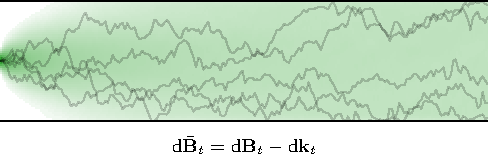
\includegraphics[width=0.49\linewidth]{images/constrained_diffusion/reflected_density.pdf}
	\hfill
	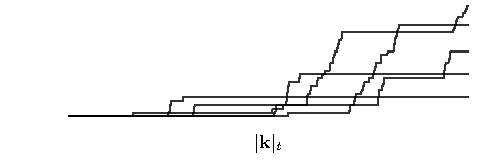
\includegraphics[width=0.49\linewidth]{images/constrained_diffusion/reflected_ks.pdf}
	\caption{\emph{Left:}
		Convergence of the reflected Brownian motion on the unit interval to the uniform distribution.
		\emph{Right:}
		Value of \(\abs{ \v{k}}_t\) for the trajectory samples on the left through time.
		}
\end{figure*}

Another approach to deal with the geometry of \(\c{M}\) is to use the standard metric \({h}\) and forward dynamics of \(\c{N}\), constraining it to \(\c{M}\) by \emph{reflecting} the process whenever it would encounter a boundary.
This results in a \emphmarginnote{reflected stochastic differential equation}.
We will first assume that \(\c{M}\) is compact and convex.
To simplify the presentation we focus on the Euclidean case \(\c{N} = \R^d\) with smooth boundary \(\partial M\)\footnote{We refer to \cref{sec:time-revers-refl} for a definition of smooth boundary.
}.

The key difference between this approach and the barrier approach is that in the reflected case we leave the geometry unchanged.
All we need to do is show that the dynamics induced by reflecting the forward process whenever it hits the boundary leads to an invariant distribution and admit a time-reversal.

It is worth noting that while barrier approaches have received considerable theoretical attention in the sampling literature \parencite{lee2017Geodesic, noble2022Barrier}, reflected methods have remained comparatively undeveloped from the methodological and practical point of view.

In the next section, we recall the technical basics of reflected stochastic processes.

\subsection{Skorokhod problem}
We define a reflected Brownian motion as the solution to the Skorokhod problem.
A solution to the \emphmarginnote{Skorokhod problem}  \parencite{skorokhod1961stochastic} consists into two coupled processes \((\bar{ \v{B}}_t, \v{k}_t)_{t \geq 0}\). \((\bar{ \v{B}}_t)_{t \geq 0}\) acts \emph{locally} as a Euclidean Brownian motion, \(( \v{B}_t)_{t \geq 0}\), and \( (\v{k}_t)_{t \geq 0}\) compensates for the excursion of \(( \v{B}_t)_{t \geq 0}\) outside the boundary so that \((\bar{ \v{B}}_t)_{t \geq 0}\) remains in \(\c{M}\).

We say that \((\bar{ \v{B}}_t, \v{k}_t)_{t \geq 0}\) is a solution to a specific {Skorokhod problem} if \(( \v{k}_t)_{t \geq 0}\) and \((\bar{ \v{B}}_t)_{t \geq 0}\) are two processes satisfying mild conditions, see \cref{sec:refl-brown-moti}, such that for any \(t \geq 0\), \begin{equation} \label{eq:rbm} \bar{ \v{B}}_t = \bar{ \v{B}}_0 + \v{B}_t - \v{k}_t \in \c{M}, \end{equation} and 
\begin{enumerate}
	\item \({\abs{ \v{k}}_t = \int_0^t \mathbf{1}_{\bar{ \v{B}}_s \in \partial \c{M}} \mathrm{d} \abs{ \v{k}}_s}\), and
	\item \({ \v{k}_t = \int_0^t \v{n}(\bar{ \v{B}}_s) \mathrm{d} \abs{ \v{k}}_s ,}\)
\end{enumerate} where \((\abs{ \v{k}}_t)_{t \geq 0}\) is the total variation of \(( \v{k}_t)_{t \geq 0}\) and \( \v{n}\) is the outward normal vector field to \(\c{M}\)\footnote{We extend the normal \( \v{n}\) to the whole space by letting \( \v{n}(x)=0\) if \(x \not \in \partial \c{M}\).
}.

When \((\bar{ \v{B}}_t)_{t \geq 0}\) hits the boundary, the first condition,  \({ \v{k}_t = \int_0^t \v{n}(\bar{ \v{B}}_s) \mathrm{d} \abs{ \v{k}}_s }\), tells us that \(- \v{k}_t\) ``compensates'' for \(\bar{ \v{B}}_t\) by pushing the process back into \(\c{M}\) along the inward normal \(- \v{n}(\bar{\v{B}}_s)\).
The second condition, \({\abs{ \v{k}}_t = \int_0^t \mathbf{1}_{\bar{ \v{B}}_s \in \partial \c{M}} \mathrm{d} \abs{ \v{k}}_s}\) can be interpreted as \( \v{k}_t\) being constant when \((\bar{ \v{B}}_t)_{t \geq 0}\) does not hit the boundary.
As a result \((\bar{ \v{B}}_t)_{t \geq 0}\) can be understood as the continuous-time counterpart to a reflected Gaussian random walk.

The process \(( \v{k}_t)_{t \geq 0}\) can be related to the notion of \emph{local time} \parencite{revuz2013continuous} and quantifies the amount of time \((\bar{ \v{B}}_t)_{t \geq 0}\) spends at the boundary \(\partial \c{M}\).
\textcite[theorem
	2.1]{lions1984stochastic} ensure the existence and uniqueness of a solution to
the Skorokhod problem.
One key observation is that the event \(\{ \bar{ \v{B}}_t \in \partial \c{M} \}\) has probability zero \parencite[Section 7, Lemma 7]{harrison1987brownian}.
As in the \emph{unconstrained} setting, one can describe the dynamics of the density of \(\bar{ \v{B}}_t\).
\begin{proposition}[Time evolution of the density of a Skorokhod problem]
	\label{prop:skorokhod_time_evolution}
	For any \(t > 0\), the distribution of \(\bar{ \v{B}}_t\) admits a density w.r.t.\
	the Lebesgue measure denoted \(p_t\).
	In addition, we have for any \(x \in \mathrm{int}(\c{M})\) and \(x_0 \in \partial \c{M}\) \begin{equation} \label{eq:heat_eq_rbm} \partial_t p_t(x) = \tfrac{1}{2} \Delta p_t(x) , \quad \partial_{ \v{n}} p_t(x_0) = 0 , \end{equation} where we recall that \(\mathbf{n}\) is the outward normal to \(\c{M}\).
\end{proposition}
\begin{proof}
	\textcite[theorem 2.2]{burdzy2004heat}
\end{proof}
Note that contrary to the unconstrained setting, the heat equation has \emph{Neumann} boundary conditions.

As a consequence of \cref{prop:skorokhod_time_evolution}, similar to the compact Riemannian setting \parencite{saloff1994precise}, it can be shown that the reflected Brownian motion converges to the uniform distribution on \(\c{M}\) exponentially fast \parencite{loper2020uniform,burdzy2006traps}, see \cref{fig:rbm}.
Hence, \((\bar{ \v{B}}_t)_{t \geq 0}\) is a candidate for a forward noising process in the context of diffusion models.

\subsection{Time-reversal}
In order to extend the diffusion model approach to the reflected setting, we need to derive \emph{time-reversal} for \((\bar{ \v{B}}_t)_{t \in \sbr{0,T}}\).
Namely, we need to characterise the evolution of \((\v{X}_t^\vsla{})_{t \in \sbr{0,T}} = (\bar{ \v{B}}_{T-t})_{t \in \sbr{0,T}}\).
It can be shown that the time-reversal of \((\bar{ \v{B}}_t)_{t \in \sbr{0,T}}\) is also the solution to a Skorokhod problem.

\begin{theorem}[Time reversal of Brownian Shorokhod problems]
	\label{sec:time-reversal-reflected}
	There exist \((\v{k}_t^\vsla{})_{t \geq 0}\) a bounded variation process and a Brownian motion \(( \v{B}_t)_{t \geq0}\) such that \begin{equation} { \v{X}_t^\vsla{} = \v{X}_0^\vsla{} + \v{B}_t + \int_0^t \nabla \log p_{T-s}({ \v{X}}^\vsla{}_s) \mathrm{d} s - \v{k}_t^\vsla{} .
	} \label{eq:rbm}
	\end{equation}
	In addition, for any \(t \in \sbr{0,T}\) we have \begin{equation} \label{eq:skorokhod_reversal} {\abs{\v{k}}_t^\vsla{} = \int_0^t \mathbf{1}_{{ \v{X}}^\vsla{}_s \in \partial \c{M}} \mathrm{d} \abs{\v{k}}_s^\vsla{} , \quad \v{k}_t^\vsla{} = \int_0^t \v{n}({ \v{X}}_s^\vsla{}) \mathrm{d} \abs{\v{k}}_s^\vsla{} .
		}
	\end{equation}
\end{theorem}
\begin{proof}
	\Cref{sec:time-revers-refl}.
\end{proof}
This proof follows \textcite{petit1997Time} which provides a time-reversal in the case where \(\c{M}\) is the positive orthant.
It is based on an extension of \textcite{haussmann1986time} to the reflected setting, with a careful handling of the boundary conditions.
In particular, contrary to \textcite{petit1997Time}, we do not rely on an explicit expression of \(p_t\) but instead use the intrinsic properties of \(( \v{k}_t)_{t \geq 0}\).

Informally, \cref{sec:time-reversal-reflected} means that the process \((\v{X}_t^\vsla{})_{t \in \sbr{0,T}}\) satisfies \begin{equation} \label{eq:evolution_Y} \mathrm{d} \v{X}_t^\vsla{} = \nabla \log p_{T-t}(\v{X}_t^\vsla{}) \mathrm{d} t + \mathrm{d} \v{B}_t - \mathrm{d} \v{k}_t^\vsla{} , \end{equation} which echoes the usual time-reversal formula of \cref{thm:fokker-plank_time_reversal_manifold}.
In practice, in order to sample from \((\v{X}_t^\vsla{})_{t \in \sbr{0,T}}\), one needs to consider the \emph{reflected} version of the \emph{unconstrained} dynamics \(\mathrm{d} \v{X}_t^\vsla{} = \nabla \log p_{T-t}(\v{X}_t^\vsla{}) \mathrm{d} t + \mathrm{d} \v{B}_t\).

\subsection{Sampling}
In practice, we approximately sample the reflected dynamics by considering the Markov chain given by \cref{alg:rrw}.
We refer to \textcite{pacchiarotti1998numerical,bossy2004symmetrized} for weak convergence results on this numerical scheme in the Euclidean setting.
This makes use of a discreted reflection step, detailed in \cref{alg:reflection}.

\begin{algorithm}[t]
	\caption[]{\protect\marginnote{Reflected random walk}Discretisation of the stochastic differential equation \(\mathrm{d} \v{X}_t = b(t, \v{X}_t) \mathrm{d} t + \mathrm{d} \v{B}_t - \mathrm{d} \v{k}_t\).
	}
	\label{alg:rrw}
	\begin{algorithmic}
		\State { \bfseries Require:} \(T\) (simulation time), \(N\) (number of steps), \(X_0^\gamma\) (initial point), \(\{f_i\}_{i \in \mathcal{I}}\) (boundary functions)
		\State \(\gamma = T / N\)
		\For{\(k \in \{0, \dots, N-1\}\)}
		\State \(Z_{k+1} \sim \mathrm{N}(0, \m{I})\)
		\State \(X_{k+1}^\gamma = \text{ReflectedStep}[X_{k}^\gamma, \sqrt{\gamma}
			Z_{k+1}, \{f_i\}_{i \in \mathcal{I}}]\) \EndFor \State { \bfseries return} \(\{ X_k^\gamma\}_{k=0}^{N}\) \end{algorithmic} \end{algorithm} 
\begin{algorithm}[t]
	\begin{algorithmic}
		\Require \(x \in \c{M}\), \(\v{v} \in \mathrm{T}_x\c{M}\), \(\{f_i\}_{i \in \mathcal{I}}\)
		\State \(\ell \gets \norm{\v{v}}_{g}\)
		\State \(\v{s} \gets \v{v} / \norm{\v{v}}_{g}\)
		\While{\(\ell \geq 0\)}
		\State \(d_i = \arg \intersect_t\sbr{\exp_{g}(x, t\v{s}), f_i}\)
		\State \(i \gets \argmin_i\; d_i \; s.t. \; d_i > 0\)
		\State \(\alpha \gets \min\del{d_i, \ell} \)
		\State \(x' \gets \exp_{g}\del{x, \alpha\v{s}}\)
		\State \(\v{s} \gets \paralleltransport_{g}\del{x, \v{s}, x'} \)
		\State \(\v{s} \gets \reflect\del{\v{s}, f_i}\)
		\State \(\ell \gets \ell - \alpha\)
		\State \(x \gets x'\)
		\EndWhile
		\State \textbf{return} \(x\)
	\end{algorithmic}
	\caption[]{
		\protect\marginnote{Reflected step algorithm}The algorithm operates by repeatedly taking geodesic steps until one of the constraints is violated or the step is fully taken.
		Upon hitting the boundary we parallel transport the tangent vector to the boundary and then reflect it against the boundary.
		We then start a new geodesic from this point in the new direction.
		The \({\arg} \intersect_t\) function computes the distance one must travel along a geodesic in direction \(\v{s}\) until constraint \(f_i\) is intersected.
		For a discussion of \(\paralleltransport\), \(\exp_{g}\) and \(\reflect\) please see \cref{def:boundary_intersection,def:manifold_reflection}.
	}
	\label{alg:reflection}
\end{algorithm}

\subsection{Extending the technical results}

In this section we have made three strong assumptions: that the underlying manifold is a Euclidean space, and that the set of constrains form a compact, convex set, and that the boundary of the set is smooth.

Relaxing the assumption that the underlying manifold is a Euclidean space seems possible as the definition of Skorokohd problems extends naturally to the Riemannian manifold setting.
The main difficulty in analysing Skorokhod problems is careful analysis of the behaviour on the boundary, which should be possible on manifolds.
There exists little literature on this topic at present, however.  

Similar to the barrier methods, relaxing the compact assumption is possible if we can factorise the space into a compact set and an unconstrained set.

Relaxing the convexity assumption is likely to be difficult, and would require significant new results on the convergence of reflected Brownian motion on non-convex sets.
This may be possible with other assumptions on the set, such as being star-shaped.

Relaxing the smoothness assumption is also likely to be very difficult as the technical complexity of dealing with such boundaries becomes high.
We note however that this is not a significant practical limitation.
For any non-smooth regions of a boundary, for example a corner, we can apply an \(\epsilon-\)smoothing to the corner to make the boundary smooth, resulting in extremely minor practical differences.

\begin{figure}[h]
	\documentclass[tikz,10pt]{standalone}
\usepackage[standalone,commands]{../../MJH}

\graphicspath{/Users/mhutchin/Documents/thesis/figures/diagrams/}

% \usepackage{tikz}
% \usetikzlibrary{positioning}

\usepackage{pgfplots}
\pgfplotsset{compat=1.17}
% \usepgfplotslibrary{external}
% \usepgfplotslibrary{groupplots}
% \usepgfplotslibrary{fillbetween}
% \usetikzlibrary{fadings}

\begin{document}
    % \tikzsetnextfilename{generative_model}
    \begin{tikzpicture}
        \node (simple) at (0,0) {
\includegraphics{/Users/mhutchin/Documents/thesis/figures/diagrams/epsilon_smooth.pdf}};
        \draw[->] (2.3,.8)   -- (2.6, 1.1);
        \node (eps) at (2.55, .85) {\(\epsilon\)};
    \end{tikzpicture}
\end{document}
	\caption{\emph{Left:} A square with non-smooth corners. \emph{Right:} A square with \(\epsilon-\)smoothed corners.}	
\end{figure}

\subsection{Likelihood evaluation}
It is possible to extend the likelihood ordinary differential equation approach to computing the likelihood of a model sample in the reflected Brownian motion case, similar to \cref{sec:likel-comp}.
% The associated ordinary differential equation was first derived in \cite{lou2023reflected}.
% The form of the ordinary differential equation and the proof that it remains in \(\c{M}\) are postponed to \Cref{sec:likel-eval}.

\begin{proposition}[Likelihood ordinary differential equation for refelcted Brownian motion]
	\label{thm:reflected_likelihood_ode}
	Assume that \(\c{M} \subset \R^d\) is a bounded open set with smooth boundary.
	Assume that \((t,x) \mapsto \nabla \log p_t(x)\) is smooth on \(\cobr{0,+\infty} \times \partial \c{M}\).

	Let \((\bar{\v{B}}_t)_{t \geq 0}\) be the reflected Brownian motion with \(\bar{\v{B}}_0 \sim p_0\) smooth and supported in \(\c{M}\).
	Let \((\v{X}_t)_{t \geq 0}\) be given for any \(t \geq 0\) by \[\mathrm{d} \v{X}_t = \tfrac{1}{2} \nabla \log p_t(\v{X}_t) \mathrm{d} t\] and \(\v{X}_0 \sim p_0\), where \(p_t\) denotes the density of \(\bar{\v{B}}_t\) w.r.t.
	the Lebesgue measure for any \(t > 0\).
	Then for any \(t \in \cbr{0,T}\), \(\bar{\mathbf{B}}_t\) and \(\mathbf{X}_t\) have the same distribution.
\end{proposition}
\begin{proof}
	\Cref{sec:likel-eval}
\end{proof}


\begin{figure*}[t] \centering \begin{minipage}[0.25\textwidth]{0.25\textwidth} 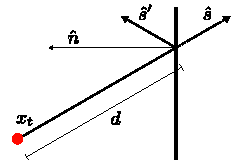
\includegraphics{images/constrained_diffusion/linear_reflection.pdf} \end{minipage} \hfill \begin{minipage}[0.25\textwidth]{0.7\textwidth} \caption{Reflection against a linear boundary.
	For a step \(s\) with magnitude \(|s|\) and direction \(\hat{s}\) the distance to the boundary described by the normal \(\hat{n}\) and offset \(b\) is \(d=\frac{\innerprod{\hat{s}}{x_t} - b}{\innerprod{\hat{s}}{\hat{n}}}\).
	The reflected direction is given by \(\hat{s}' = \hat{s} - 2\innerprod{\hat{s}}{\hat{n}}\hat{n}\).
}
\label{fig:reflection_diagrams_lin}
\end{minipage}
\vspace{1em}
\begin{minipage}{0.25\textwidth}
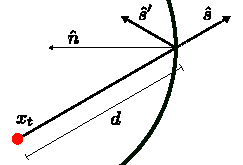
\includegraphics{images/constrained_diffusion/sphere_reflection.pdf}
\end{minipage}
\hfill
\begin{minipage}{0.7\textwidth}
\caption{Reflection against a spherical boundary.
For a sphere of radius \(r\), the distance to the boundary from \(x_t\) in direction \(s\) is given by \(d= \frac{1}{2}(\innerprod{\hat{s}}{x_t}^2 + 4 (r^2 - \norm{x_t}^2))^{1/2} -\frac{1}{2}\innerprod{\hat{s}}{x_t}\).
The normal at the intersection can be computed as the unit vector in the direction \(-2(d\hat{s} + x_t)\), and then \(\hat{s}'\) as above.
}
\label{fig:reflection_diagrams_sph}
\end{minipage}
\end{figure*}


\section{Training and parametrising score functions for constrained diffusions}
\label{sec:score-netw-param}

In order to train log-barrier and reflected diffusion models we need a \emph{tractable} score matching loss on constrained manifolds.
We will prove that the implicit score-matching loss can be extended to the constrained manifold setting so long as we enforce that the score is zero on the boundary.
This proof holds for both the log-barrier and the reflected process.

\begin{proposition}[Implicit score-matching on constrained domains]
	Let \(s \in \mathrm{C}^\infty(\cbr{0,T} \times \R^d, \R^d)\) such that for any \(x \in \partial \c{M}\) and \(t \geq 0\), \(s_t(x) =0\).
	Then, there exists \(C >0\) such that \begin{equation} {\E\sbr{\norm{\nabla \log p_t - s_t}^2} = \E\sbr{\norm{s_t}^2 + 2~ \mathrm{div}(s_t)}} + C , \end{equation} where \(\mathbb{E}\) is taken over \(\v{X}_t \sim p_t\) and \(t \sim \mathcal{U}([0,T])\).
\end{proposition}
\begin{proof}
	\Cref{app:proof_for_ism}
\end{proof}

This result immediately implies we can optimise the score network approximate the score function using the implicit score matching loss function so long as we enforce a Neumann boundary condition.

Following \textcite{liu2022estimating} we can accommodate this boundary condition in our score parameterisation by scaling the score output of the neural network by a monotone function \(h(d(x, \partial \c{M}))\) where \(d\) is the distance from \(x\) to the boundary, where \(h(0) = 0\).
In particular, we use a clipped ReLU function: \(s_\theta(t, x) = \min(1, \textrm{ReLU}(d(x, \partial \c{M}) - \delta)) \cdot \textrm{NN}_\theta(t, x)\) with \(\delta>0\) a threshold so the model is forced to be zero ``close'' to the boundary as well as exactly on the boundary. %, see \Cref{sec:exp_details} for an illustration.
The inclusion of this scaling function is necessary to produce reasonable results as we show in \cref{sec:boundary_score}.
%  The weighting function in (\ref{eq:implicit_sm}) is set to \(\lambda_t = (t + 1)\).

The forward processes (\cref{eq:langevin_hessian_manifold}) and (\cref{eq:rbm}) for the barrier and reflected methods cannot be sampled in closed form, so at training time samples from the conditional distributions \(p(\v{X}_t|\v{X}_0)\) are obtained by discretising these processes.
To take the most of this computational overhead, we use several samples from the discretised forward trajectory \((\v{X}_{t_1}, \cdots, \v{X}_{t_k}|\v{X}_0)\) instead of only using the last sample.

\section{Related work for sampling on constrained manifolds.}
Sampling from a distribution on a space defined by a set of constraints is an important ingredient in several computational tasks, such as computing the volume of a polytope \parencite{lee2017Geodesic}.
Incorporating such constraints inside MCMC algorithms while preserving fast convergence properties is an active field of research \parencite{kook2022sampling,lee2017Geodesic,noble2022Barrier}.
In this work, we are interested in sampling from the uniform distribution defined on the constrained set in order to define a proper \emph{forward process} for our diffusion model.
Log-barrier methods such as the Dikin walk or Riemannian Hamiltonian Monte Carlo \cite{Kannan2009,lee2017Geodesic,noble2022Barrier} change the geometry of the underlying space and define stochastic processes which never violate the constraints, see \cite{Kannan2009,noble2022Barrier} for instance.
If we keep the Euclidean metric, then \emph{unconstrained} stochastic processes might not be well-defined for all times.
To counter this effect, it has been proposed to \emph{reflect} the Brownian motion \cite{williams1987Reflected,petit1997Time,shkolnikov2013Timereversal}.
Finally, we also highlight hit-and-run approaches \parencite{Smith1984,Lovasz2006} which generalise Gibbs' algorithm and enjoy fast convergence properties provided that one knows how to sample from the one-dimensional marginals.


\section{Experimental results}
\label{sec:experiments-constrained}
\label{sec:diff_methods}

To demonstrate the practical utility of the constrained diffusion models introduced in \cref{sec:bsgm,sec:rbm}, we evaluate them on a series of increasingly difficult synthetic tasks on convex polytopes, including the hypercube and the simplex, in \cref{subsec:synthetic_data}.
We then highlight their applicability to real-world settings by considering two problems from robotics and protein design.
In particular, we show that our models are able to learn distributions over the space of \(d\times d\) symmetric positive definite (SPD) matrices \(S_{++}^d\) under trace constraints in \cref{subsec:psd_matrices}.
This setting that is essential to describing and controlling the motions and exerted forces of robotic platforms \parencite{yoshikawa1985manipulability}.
In \cref{subsec:protein_loops}, we use the parametrisation introduced in \textcite{han2006inverse} to map the problem of modelling the conformational ensembles of loops of proteins with fixed endpoints to the product manifold of a convex polytope and a torus.

We refer to \cref{sec:exp_details} for more details on the experimental setup.
The code used for the experiments in this chapter can be found at \url{https://github.com/oxcsml/constrained-diffusion}.

\subsection{Method characterisation on convex polytopes}
\label{subsec:synthetic_data}
\setlength{\tabcolsep}{11pt}
\begin{table*}[t]
	\centering
	\caption{
		MMD metrics between samples from synthetic distributions and trained constrained and unconstrained (Euclidean) diffusion models.
		Means and confidence intervals are computed over 5 different runs.
	}
	\label{tab:synthetic_polytope}
	\begin{tabular}{cccccccc}
		\toprule
		\multirow{2}{*}{\scshape{Space}}      & \multirow{2}{*}{\(d\)} & \multicolumn{2}{c}{\scshape{Log-barrier}} & \multicolumn{2}{c}{\scshape{Reflected}} & \multicolumn{2}{c}{\scshape{Euclidean}}                                                                \\
		                            &                      & \textsc{MMD}                    & \% in \(\mathcal{M}\)           & \textsc{MMD}                  & \% in \(\mathcal{M}\) & \textsc{MMD}     & \% in \(\mathcal{M}\) \\
		\midrule
		\multirow{3}{*}{\([-1,1]^d\)} & 2                    & \(.066 \pm{.006}\)                & 100.0                         & \(.055 \pm{.015}\)              & 100.0               & \(.062 \pm{.011}\) & 98.8                \\
		                            & 3                    & \(.209 \pm{.077}\)                & 100.0                         & \(.080 \pm{.004}\)              & 100.0               & \(.076 \pm{.004}\) & 98.5                \\
		                            & 10                   & \(.330 \pm{.004}\)                & 100.0                         & \(.313 \pm{.048}\)              & 100.0               & \(.081 \pm{.005}\) & 96.4                \\
		\midrule
		\multirow{3}{*}{\(\Delta^d\)} & 2                    & \(.050 \pm{.012}\)                & 100.0                         & \(.043 \pm{.002}\)              & 100.0               & \(.055 \pm{.013}\) & 96.4                \\
		                            & 3                    & \(.238 \pm{.009}\)                & 100.0                         & \(.181 \pm{.007}\)              & 100.0               & \(.068\pm{.014}\)  & 96.3                \\
		                            & 10                   & \(.275 \pm{.015}\)                & 100.0                         & \(.290 \pm{.009}\)              & 100.0               & \(.060	\pm{.003}\) & 92.6                \\
		\bottomrule
	\end{tabular}
\end{table*}

\begin{figure}[t]
	\begin{subfigure}{0.8\linewidth}
		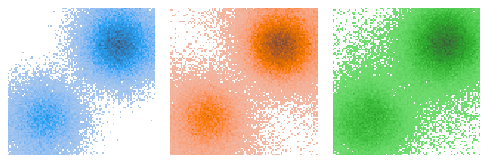
\includegraphics[width=\textwidth]{images/constrained_diffusion/toy_cube.pdf}
		\put(-250,-10){Data}
		\put(-170,-10){Log-barrier}
		\put(-70,-10){Reflected}
		\caption{2D square data.}
	\end{subfigure}
	\\
	\begin{subfigure}{0.8\linewidth}
		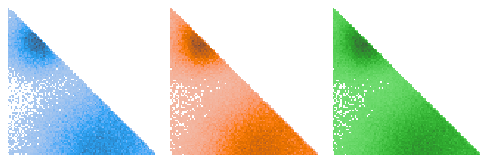
\includegraphics[width=\textwidth]{images/constrained_diffusion/toy_dirichlet.pdf}
		\put(-250,-10){Data}
		\put(-170,-10){Log-barrier}
		\put(-70,-10){Reflected}
		\caption{2D Dirichlet data.}
	\end{subfigure}
	\caption{
		Histograms of samples from the data distribution and from trained constrained diffusion models.
	}
	\label{fig:polytope_synthetic}
\end{figure}

First, we aim to assess the empirical performance of our methods on constrained manifolds of increasing dimensionality.
For this, we focus on polytopes and construct synthetic datasets that represent bimodal distributions.
In particular, we investigate two specific instances of polytopes: hypercubes and simplices.
In \cref{sec:app_synthetc_data} we also present results on the Birkhoff polytope.
We quantify the performance of each model via the Maximum Mean Discrepancy (\textsc{MMD}) \parencite{gretton2012kernel}, which is a kernel-based metric between distributions.
We present a qualitative comparison of the logarithmic barrier and reflected Brownian motion models in \cref{fig:polytope_synthetic}, and observe that both methods recover the data distribution on the two-dimensional hypercube and simplex, although the reflected method produces a better fit.
In \cref{tab:synthetic_polytope}, we report the \textsc{MMD} between the data distribution and the learnt diffusion models across a range of dimensions.
Here, we similarly observe that the reflected method consistently yields better results than the log-barrier one.

In addition, we compare both of these models to unconstrained Euclidean diffusion models.
We note that they are outperformed by the constrained models in lower dimensions, but generate better results in higher dimensions.
In contrast, however we do see that the unconstrained models do not keep their modelled density inside the boundary, and this gets worse with increasing dimension.
There are a number of potential explanations for this: First, we note that the mixture of Normal distributions we use as a synthetic data-generating process places significantly less probability mass near the boundary as its dimensionality increases, more closely resembling an unconstrained mixture distribution that is easier for the Euclidean diffusion models to learn, while posing a challenge to the log-barrier and reflected diffusion models that initialise at the uniform distribution within the constraints.
Additionally, we note that the design space and hyperparameters used for all experiments were informed by best practices for Euclidean models that may be suboptimal for the more complex dynamics of constrained diffusion models.

\subsection{Modelling robotic arms under force and velocity constraints}
\label{subsec:psd_matrices}

\begin{figure}[t]
	\centering
	\begin{subfigure}{0.22\columnwidth}
		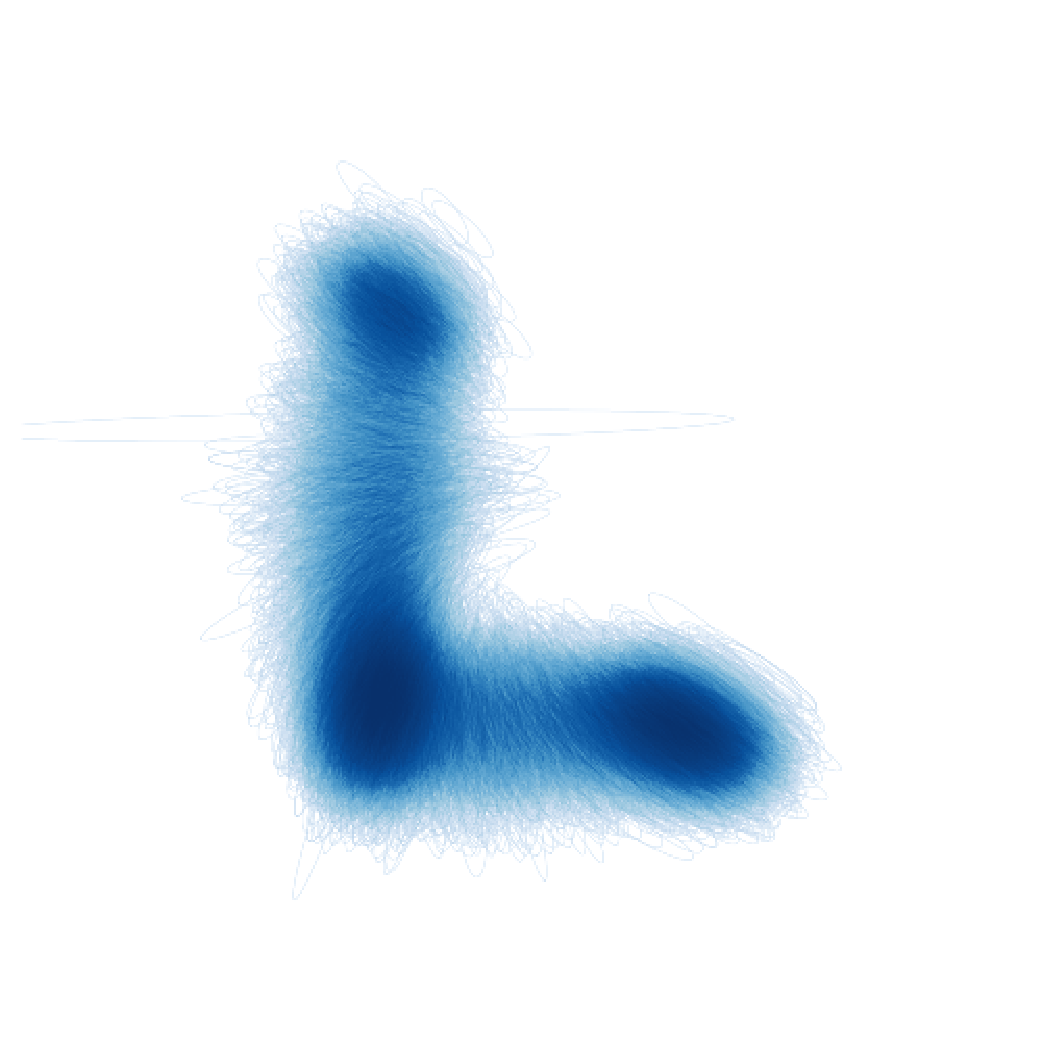
\includegraphics[width=\linewidth]{images/constrained_diffusion/spd_l_data.pdf}
		\caption{Samples from the data distribution.}
	\end{subfigure}
	\hfill
	\begin{subfigure}{0.22\columnwidth}
		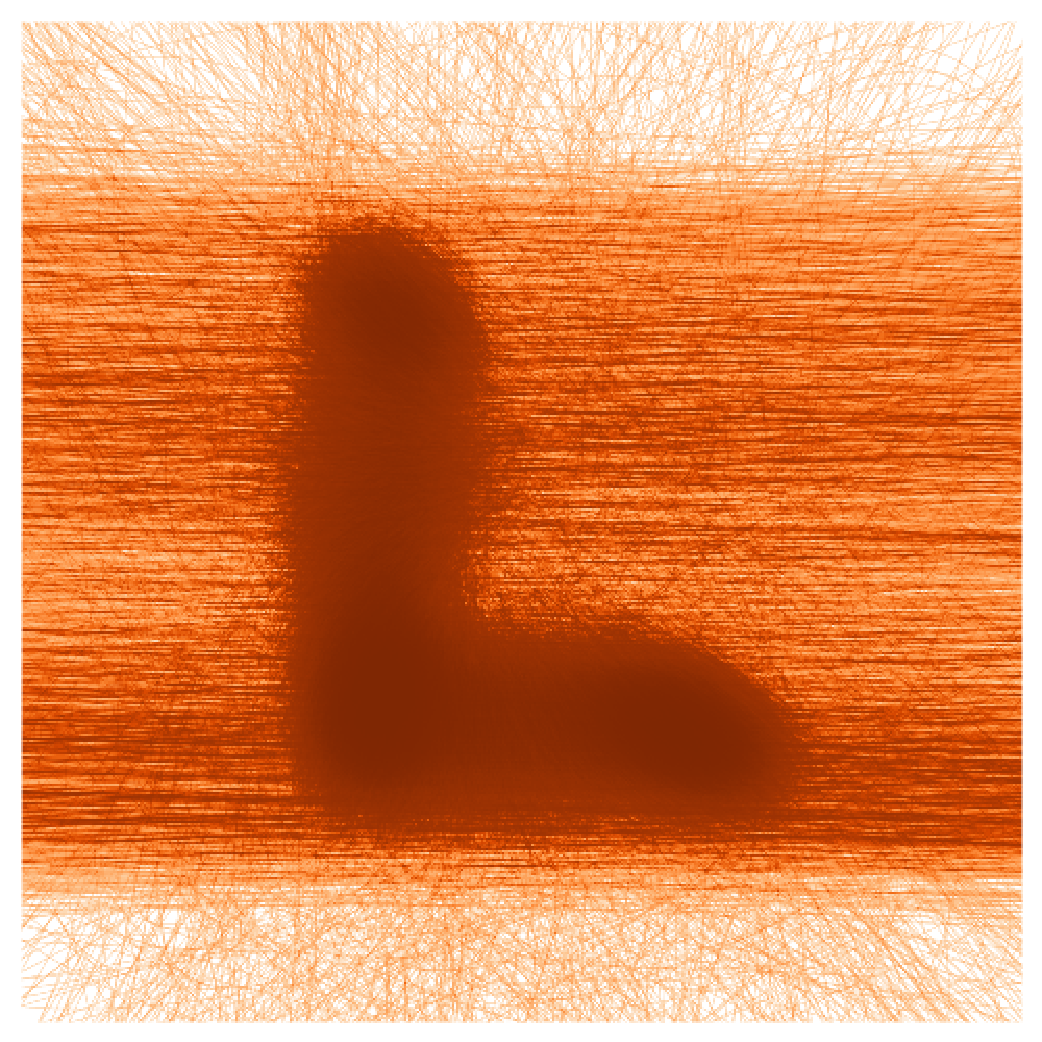
\includegraphics[width=\linewidth]{images/constrained_diffusion/spd_l_logbarrier.pdf}
		\caption{Samples from our log-barrier diffusion model.}
	\end{subfigure}
	\hfill
	\begin{subfigure}{0.22\columnwidth}
		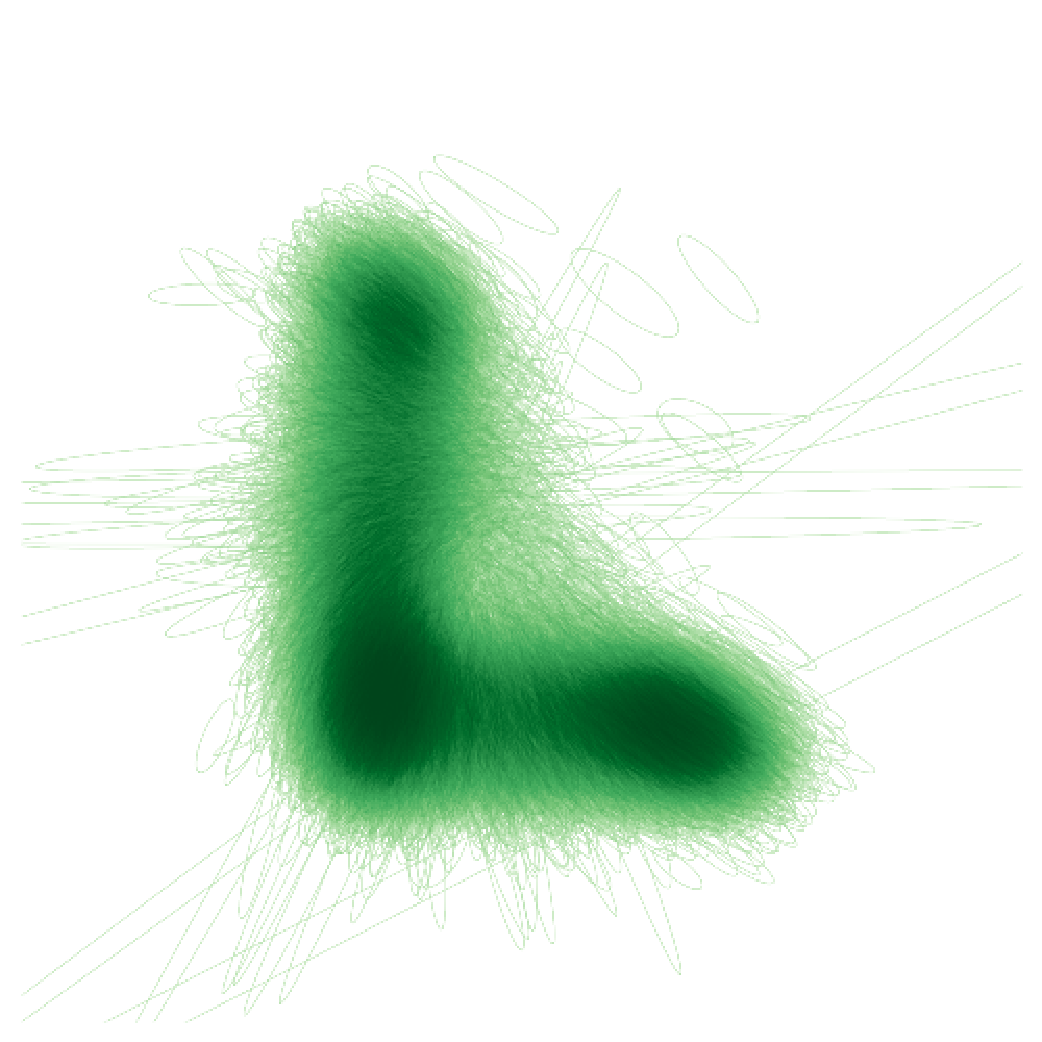
\includegraphics[width=\linewidth]{images/constrained_diffusion/spd_l_reflected.pdf}
		\caption{Samples from our reflected diffusion model.}
	\end{subfigure}
	\hfill
	\begin{subfigure}{0.22\columnwidth}
		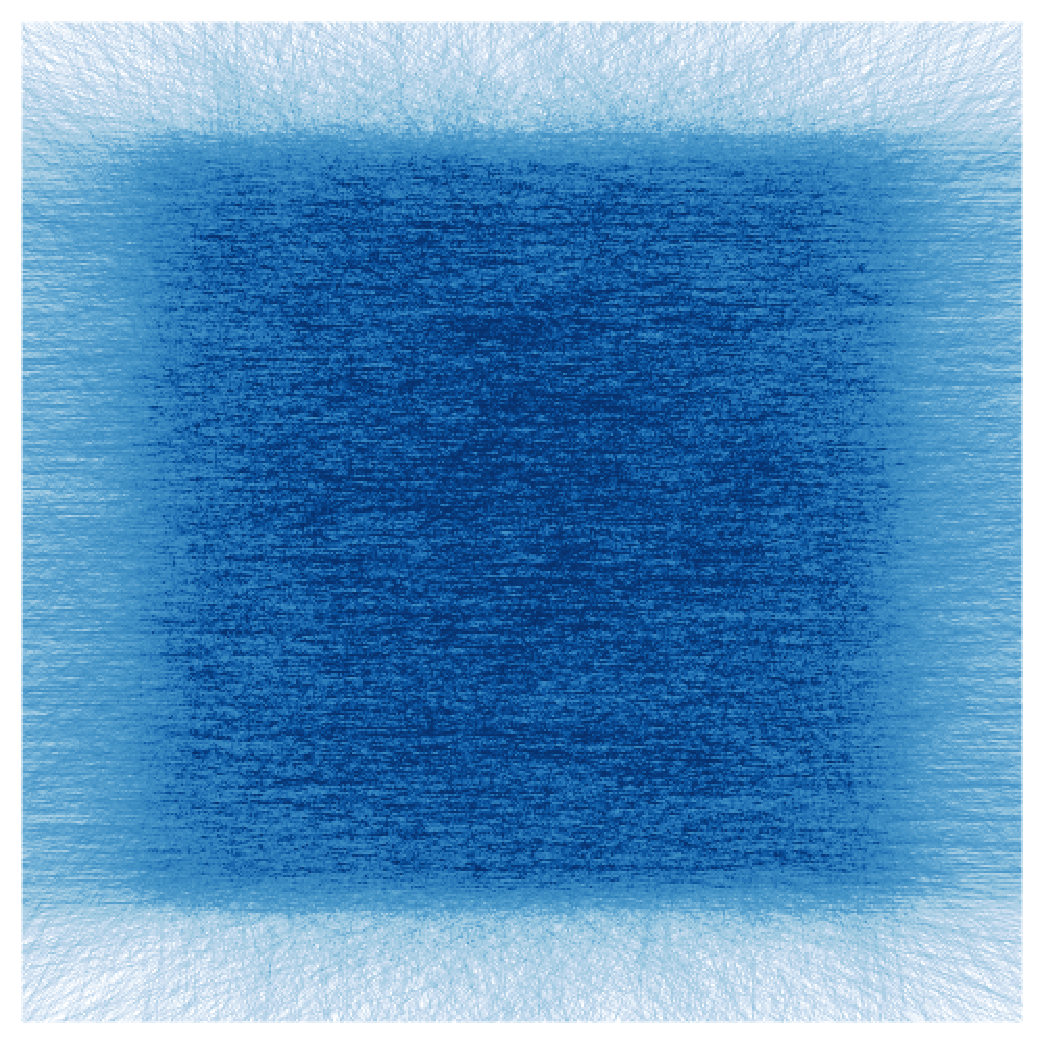
\includegraphics[width=\linewidth]{images/constrained_diffusion/spd_l_uniform.pdf}
		\caption{Samples from the uniform distribution.}
	\end{subfigure}
	\caption{Samples in \(S_{++}^2\times\mathbb{R}^2\) from (a) the data distribution, (b) our log-barrier diffusion model, (c) our reflected diffusion model and (d) the uniform distribution.
		Each sample is visualised as the manipulability ellipsoid encoded by the SPD matrix \(M\in S_{++}^2\) placed at the corresponding location in \(\mathbb{R}^2\).
		Additional results and full correlation plots are postponed to~\cref{sec:app_spd_exp}.
	}
	\label{fig:spd_data}
\end{figure}

Accurately determining and controlling the movement and exerted forces of robotic platforms is a fundamental problem in many real-world robotics applications.
A kinetostatic descriptor that is commonly used to quantify the ability of a robotic arm to move and apply forces along certain dimensions is the so-called \emphmarginnote{manipulability ellipsoid} \(E\in\mathbb{R}^d\) \parencite{yoshikawa1985manipulability} which is naturally described as a symmetric positive definite (SPD) matrix \(\mathrm{M} \in\mathbb{R}^{d\times d}\) \parencite{jaquier2021geometry}.
The manifold of such \(d\times d\) SPD matrices, denoted as \(S_{++}^d\), is defined as the set of matrices \( \{ x^\top \mathrm{M} x \geq 0 , \ x\in \mathbb{R}^d : \mathrm{M} \in \R^{d \times d} \} \).

In many practical settings, it may be desirable to constrain the volume of \(E\) to retain flexibility or limit the magnitude of an exerted force, which can be expressed as an upper bound on the trace of \(\mathrm{M}\), i.e. as the inequality constraint \(\sum_{i=1}^d \mathrm{M}_{ii} < C\) with \(C >0\).
Constraining the rest of the entries of the matrix to ensure it is SPD is non-trivial.

Alternatively, we can parameterise the SPD matrices via their Cholesky decomposition.
Each SPD matrix has a unique decomposition of the form \(\mathrm{M} = \mathrm{L} \mathrm{L}^\top\), where \( \mathrm{L}\) is a lower triangular matrix with strictly positive diagonal \parencite[p.143]{golub2013matrix}.
Constraining the entries of this matrix simply requires ensuring the diagonal is positive.
The trace of the SPD matrix is given by \(\mathrm{Tr}(\mathrm{M}) = \mathrm{Tr}(\mathrm{L} \mathrm{L}^\top) = \sum_{ij}\mathrm{L}_{ij}^2\), and results in the constraint on the entries of \(\mathrm{L}\) to live in a ball of radius \(C\).
We additionally model the two-dimensional position of the arm.

In summary, the space over which we parameterise the diffusion models is defined as \[\sbr{ \mathrm{L} \in \R^{d(d+1)/2} : \mathrm{L}_{i,i} > 0, \sum_{i,j} \mathrm{L}_{i,j}^2 < C } \times \R^2.\]
Under the Euclidean metric, we can apply both our log-barrier and reflected approaches.
The positive diagonal (linear) constraint is handled similarly to the polytope setting.
The reflection on the ball boundary is defined and illustrated on \cref{fig:reflection_diagrams_lin,fig:reflection_diagrams_sph}.

Using this framework, we model the datasets presented in \textcite{jaquier2021geometry}.
This consists of demonstrations of a robotic arm drawing different letters in the plane, providing the respective positional trajectories (\(\mathbb{R}^2\)) and velocity manipulability ellipsoids (\(S^2_{++}\)).

We use the processing routines provided by \textcite{jaquier2021geometry} to interpolate the trajectories into \(10^4\) distinct points, for each of which we derive the position \(\mathbf{x}\in\mathbb{R}^2\) and the PSD matrix \( e \in S^2_{++}\).
parametrising the velocity manipulability ellipsoid \(M\in\mathbb{R}^2\).
The resulting data is split into training, validation, and test sets by trajectory.
We add a small amount of Gaussian noise to these trajectories.

We visualise samples from this distribution as ellipsoids respecting the SPD matrix placed at a point in the plane.
The dataset, samples from the trained log-barrier and reflected diffusion models, and the uniform distribution are shown in \cref{fig:spd_data}.
We qualitatively observe that the reflected method is able to fit the joint data distribution better than the log-barrier method.
Quantitatively, the reflected method achieves an MMD of 0.161 with respect to the dataset as opposed to 0.247 for the log-barrier method.

\subsection{Modelling protein loops with anchored endpoints}
\label{subsec:protein_loops}

Polypeptides and proteins constitute an important class of biogenic macromolecules that underpin most aspects of organic life.
Accurately modelling their conformational ensembles,i.e. the set of three-dimensional structures they assume under physiological conditions, is essential to both understanding the biological function of existing and designing the enzymatic or therapeutic properties of novel proteins \parencite{lane2023protein}.
Motivated by the success of diffusion models in computer vision and natural language processing, there has been considerable interest in applying them to learn and sample from distributions over the conformational space of protein structures \parencite{watson2022Broadly, trippe2022Diffusion, wu2022protein}.

\subsubsection{Problem parameterisation}
\label{sec:protein_param}

Proteins are biopolymers in which a sequence of \(N\) amino acids is joined together through \(N-1\) peptide bonds, resulting in a so-called polypeptide backbone with protruding amino acid residues.
As the deviation of chemical bond lengths and angles from their theoretical optimum is generally negligible, the problem of modelling the three-dimensional structure of this polypeptide chain is often reframed in the space of the internal torsion angles \(\Phi\) and \(\Psi\), see~\cref{fig:peptide_chain} for an illustration, which can be modelled on a \((2N-2)\)-dimensional torus \(\mathbb{T}^{2N-2}\).

\begin{figure}[h]
	\centering
	\begin{subfigure}[t]{0.48\textwidth}
		\centering
		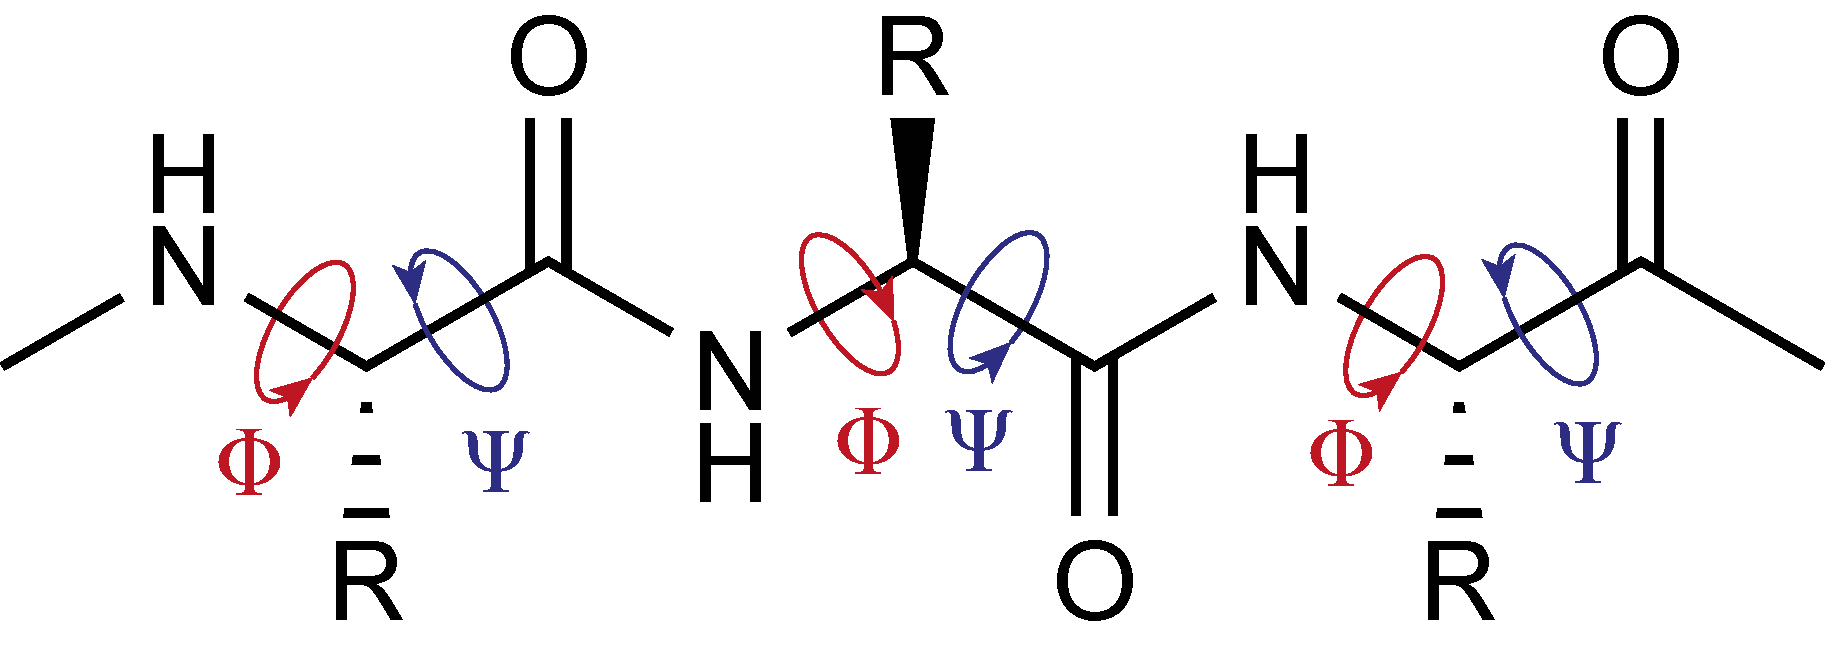
\includegraphics[width=\linewidth]{images/constrained_diffusion/peptide_chain.pdf}
		\caption{A commonly-used approximate parameterisation of backbone geometry only considers the \(C_\alpha\) torsion angles \(\Phi\) and \(\Psi\).}
		\label{fig:peptide_chain}
	\end{subfigure}
	\hfill
	\begin{subfigure}[t]{0.48\textwidth}
		\centering
		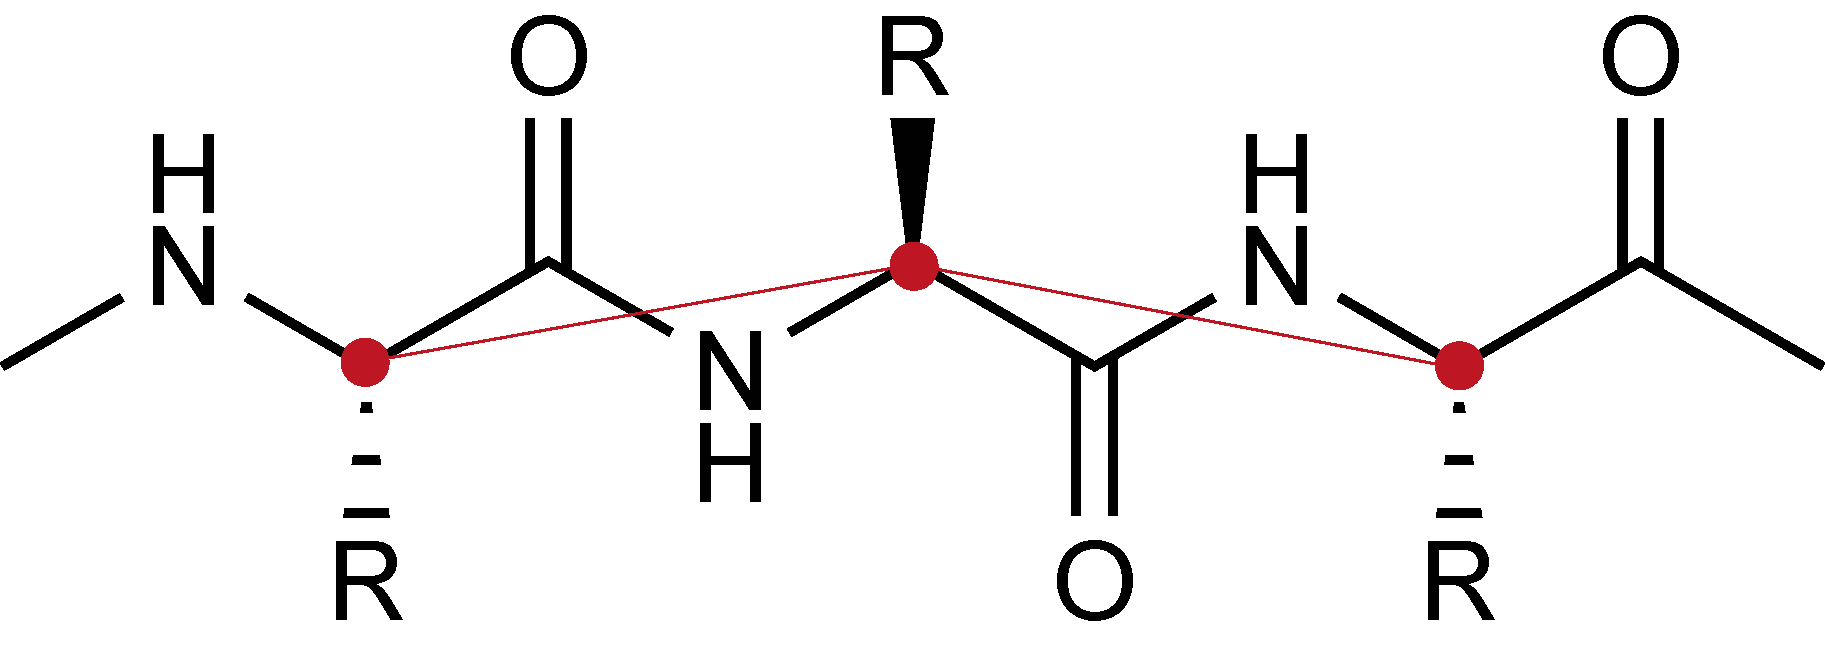
\includegraphics[width=\linewidth]{images/constrained_diffusion/ca_trace.pdf}
		\caption{As peptide bond orientations can be inferred relatively reliably, researchers often only model the \(C_\alpha\) traces.}
		\label{fig:peptide_trace}
	\end{subfigure}
	\caption{Standard approaches to modelling the conformations of polypeptide backbones.}
	\label{fig:peptide}
\end{figure}

In many data-scarce settings such as antibody or enzyme design, it is often unnecessary or even undesirable to model the structure of an entire protein, as researchers are primarily interested in specific functional sites with distinct biochemical properties.
However, generating conformational ensembles for such substructural elements necessitates positional constraints on their endpoints to ensure that they can be accommodated by the remaining protein scaffold.
While it is conceivable that a diffusion model could derive such constraints from limited experimental data, we argue that it is much more efficient and precise to encode them explicitly.

For this purpose, we adopt the distance constraint formulation from \textcite{han2006inverse} and interpret the backbone as a spatial chain with \(N\) spherical joints and fixed-length links, see~\cref{fig:cyclic_peptide} for an illustration.
After selecting a suitable anchor point, the geometry of the polypeptide chain is fully specified by \begin{enumerate*}[label=(\alph*)] \item the set of link lengths \(\mathbf{\ell}=\{\ell_j\}_{j=1}^{N}\), \item the set of vectors \(\mathbf{r}=\{r(1,j)\}_{j=2}^{N}\) between the anchor point and each atom in the chain, and \item the set of dihedral angles\end{enumerate*} \[ \mathbf{T}=\left\{\arccos\left(\frac{\vert\langle r(1,j)\times r(1,j+1), r(1,j+1)\times r(1,j+2)\rangle\vert}{\vert r(1,j)\times r(1,j+1)\vert\vert r(1,j+1) r(1,j+2)\vert}\right)\right\}_{j=2}^{N-2}\in\mathbb{T}^{N-3} \] between any three consecutive vectors.
After specifying the fixed bond lengths \(\ell\), including an arbitrary anchor point distance \(d_\text{anchor}=\ell_N=r(1,N)\), the set of valid vectors \(\mathbf{r}\) is given by the convex polytope \(\mathbb{P}\subseteq\mathbb{R}^{N-3}\) defined by the following linear constraints (see~\cref{fig:convex_polytope_loop_illustration} for an illustration): 
\[ 
	\begin{array}{rcl} r(1,3) & \leq & \ell_1+\ell_2 , \\ -r(1,3) & \leq & -\left|\ell_1-\ell_2\right|, \\ 
	\end{array} 
	\\
	\left.
	\begin{array}{rcl}
		r(1, j)-r(1, j+1)  & \leq & \ell_j,  \\
		-r(1, j)+r(1, j+1) & \leq & \ell_j,  \\
		-r(j)-r(j+1)       & \leq & -\ell_j,
	\end{array}\right\}3 \leq j \leq N-2,
	\\
	\begin{array}{rcl}
		r(1, N-1)  & \leq & \ell_{N-1}+d_\text{anchor},               \\
		-r(1, N-1) & \leq & -\left|\ell_{N-1}-d_\text{anchor}\right|.
	\end{array}
\]
\begin{figure}[t]
	\centering
	\begin{subfigure}[t]{0.45\textwidth}
		\centering
		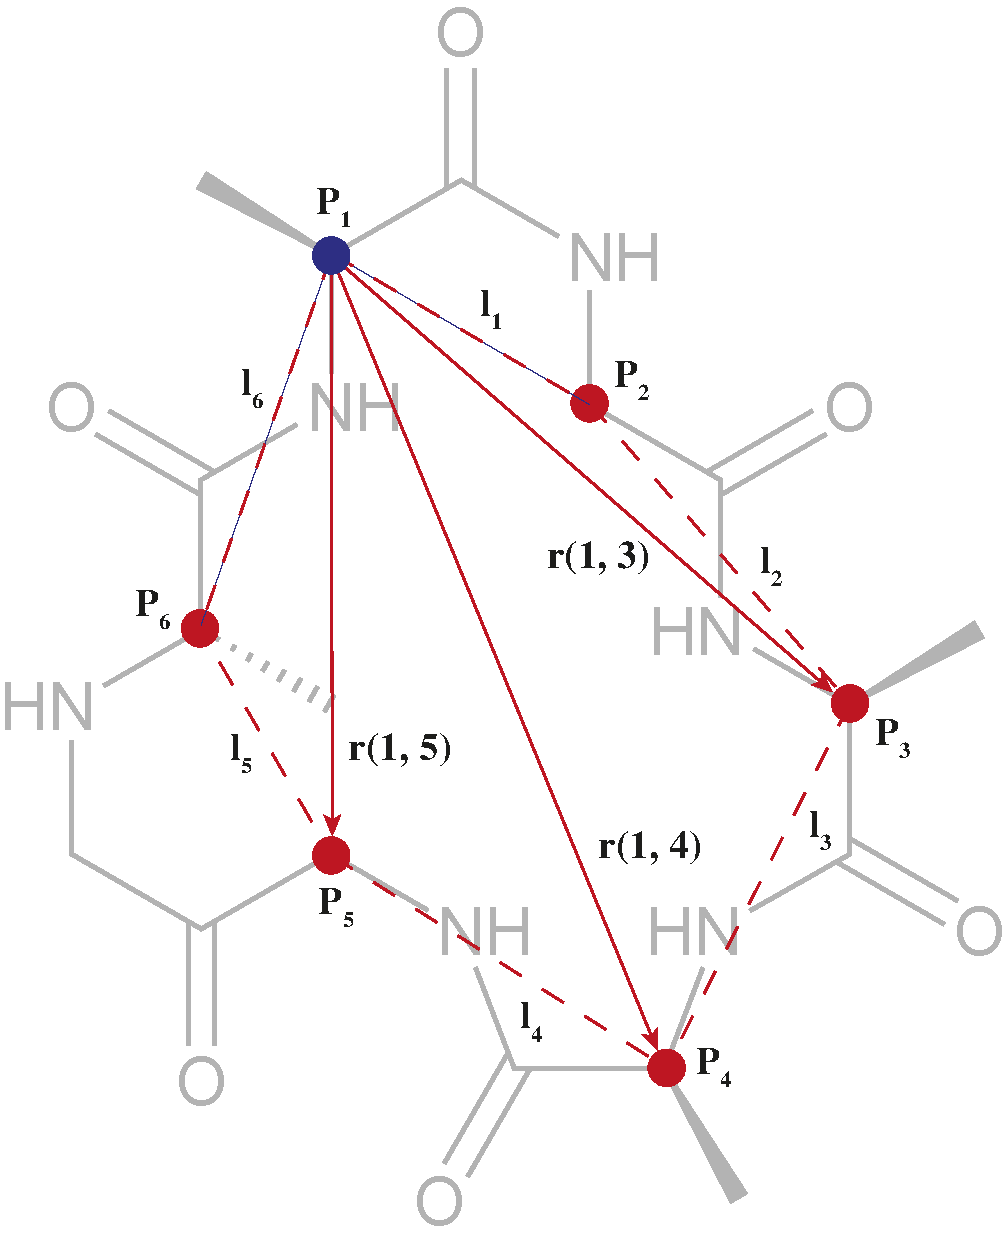
\includegraphics[width=0.7\linewidth]{images/constrained_diffusion/cyclic_peptide.pdf}
		\caption{An illustrative diagram of the proposed parameterisation for modelling the \(C_\alpha\) trace geometry of the cyclic peptide \textsc{c-AAGAGG}.}
		\label{fig:cyclic_peptide}
	\end{subfigure}
	\hfill
	\begin{subfigure}[t]{0.45\textwidth}
		\centering
		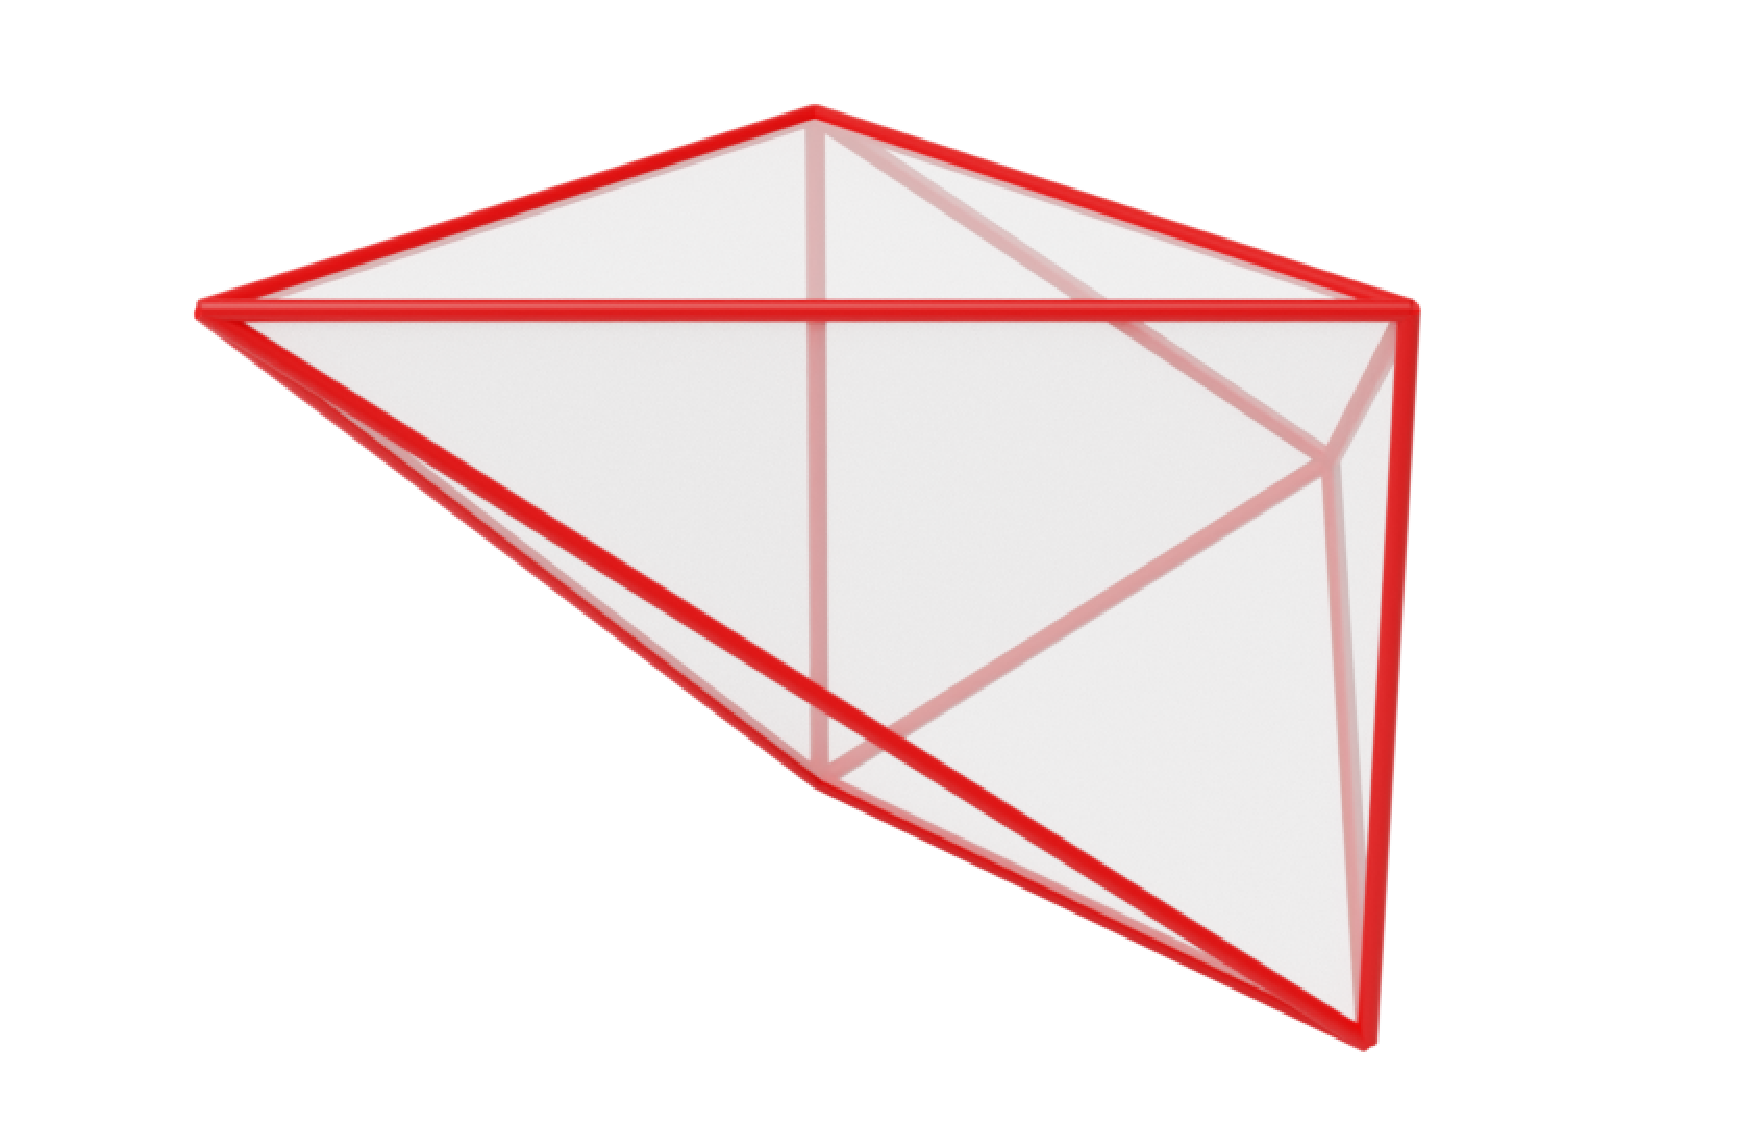
\includegraphics[width=\linewidth]{images/constrained_diffusion/hull.pdf}
		\caption{The convex polytope constraining the diagonals of the triangles for the given bond lengths in the illustrated molecule.
			The total design space is the product of this polytope with the 4D flat torus.
		}
		\label{fig:convex_polytope_loop_illustration}
	\end{subfigure}
	\caption{Parameterising the conformational space of polypeptide backbones under anchor point distance constraints.}
	\label{fig:han_and_rudolph_rep}
\end{figure}

This means that the set of all valid polypeptide backbone conformations is defined by the product manifold \(\mathbb{P}\times\mathbb{T}^{N-3}\), enabling us to train diffusion models that exclusively generate conformations with a fixed anchor point distance \(d_\text{anchor}\).

\subsubsection{Data generation}
\label{sec:protein_data}

As a proof-of-concept for the practicality of our methods, we chose to model the conformational distribution of the cyclic peptide \textsc{c-AAGAGG}.
Cyclic peptides are an increasingly important drug modality with therapeutic uses ranging from antimicrobials to oncology, exhibiting circular polypeptide backbones (i.e. \(d_\text{anchor}=0\)) that confer a range of desirable pharmacodynamic and pharmacokinetic properties \parencite{dougherty2019understanding}.
To reduce the dimensionality of the problem, we only consider the \(C_\alpha\) traces (with fixed \(C_\alpha\)-\(C_\alpha\) link distances of 3.6 \AA) instead of the full polypeptide backbone (see \cref{fig:peptide_trace}), although we note that our framework is applicable to both settings.

To derive a suitable dataset, the product manifold \(\mathbb{P}\times\mathbb{T}^3\) describing the conformations of cyclic \(C_\alpha\) traces of length \(N=6\) was constructed, see~\cref{fig:cyclic_peptide,fig:convex_polytope_loop_illustration} for an illustration, and used to generate \(10^7\) uniform samples satisfying the anchor point distance constraint \(d_\text{anchor}=0\).
Subsequently, an estimate of the free energy \(E_i\) of each sample \(i\) was obtained by (1) reconstructing the full-atom peptide from each \(C_\alpha\) trace using the \textsc{PULCHRA} algorithm \parencite{rotkiewicz2008fast}, (2) relaxing all non-\(C_\alpha\) backbone and side-chain atoms (keeping the \(C_\alpha\) positions fixed), and (3) quantifying the potential energy of each of the resulting conformations using the \textsc{OpenMM} suite of molecular dynamics tools \parencite{eastman2017openmm}, and the \textsc{AMBER} force field \parencite{hornak2006comparison}.
These free energy estimates were then used to approximate the Boltzmann distribution over conformational states \[ \textstyle{ p_B(i) \propto \exp\left(-\frac{E_i}{k_BT}\right),} \] where temperature was set to \(T=\SI{273.15}{\kelvin}\) and \(k_B=\SI{1.380649e-23}{\joule\per\kelvin}\) is the Boltzmann constant.
We then apply a very minor amount of smoothing to the resulting distribution by running forward Brownian motion on both the polytope and the torus for 10 steps, using a small step size of \(\num{5e-3}\) and the respective metrics.
Finally, a subsample of \(10^6\) \(C_\alpha\) traces was drawn from this distribution and used for training and evaluating our models.

\subsubsection{Modelling the problem}
% \begin{figure}[t]
% 	\centering
% 	\vspace{-0.5cm}
% 	\begin{subfigure}[t]{0.45\textwidth}
% 		\centering
% 		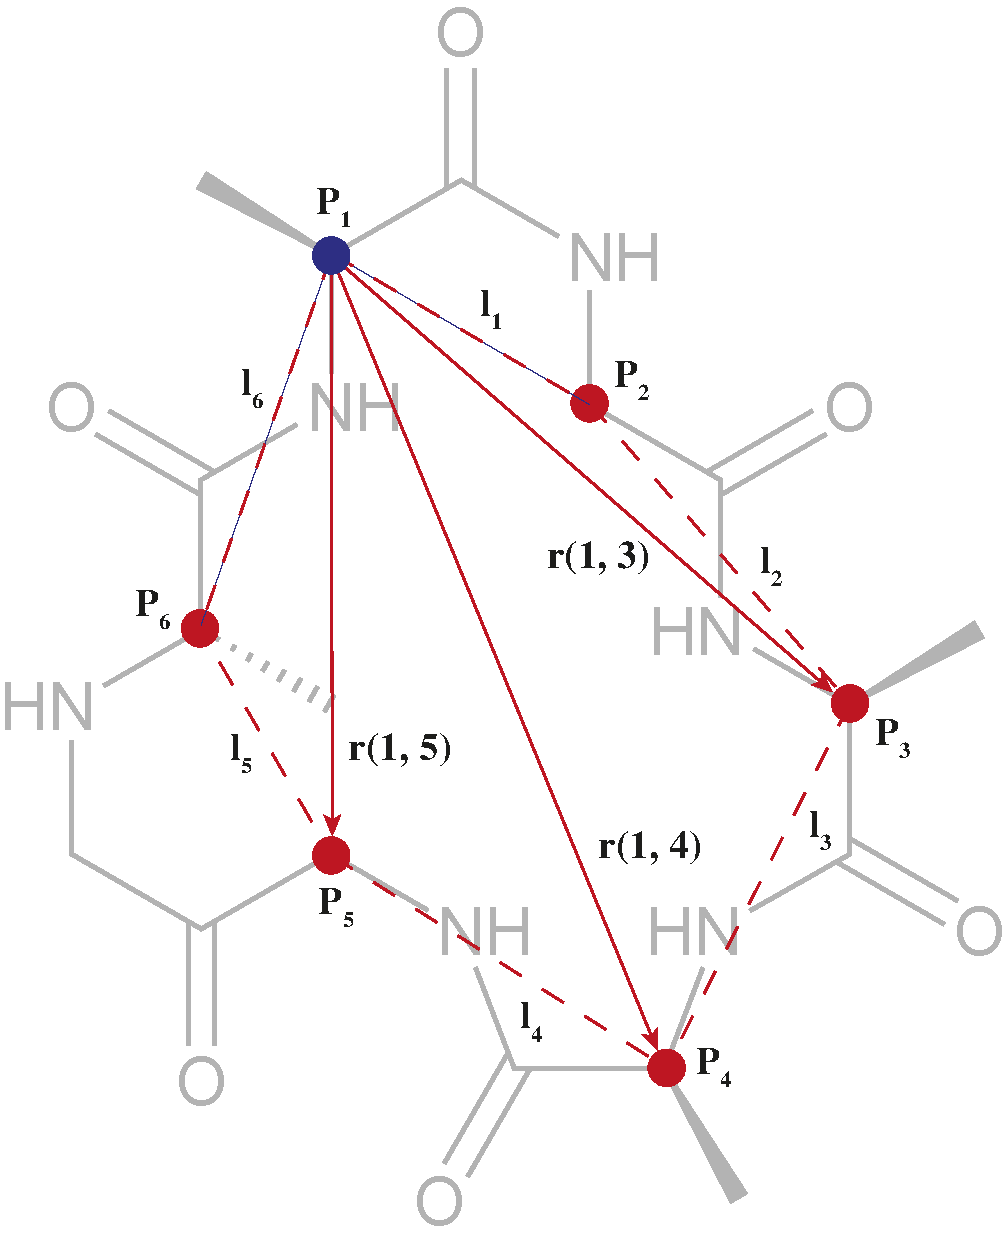
\includegraphics[height=4cm]{images/constrained_diffusion/cyclic_peptide.pdf}
% 		\caption{An illustrative diagram of the parameterisation used for the conformational modelling of the \(C_\alpha\) trace of a cyclic peptide, introduced in \cite{han2006inverse}.}
% 		\label{fig:cyclic_peptide_main}
% 	\end{subfigure}
% 	\hfill
% 	\begin{subfigure}[t]{0.45\textwidth}
% 		\centering
% 		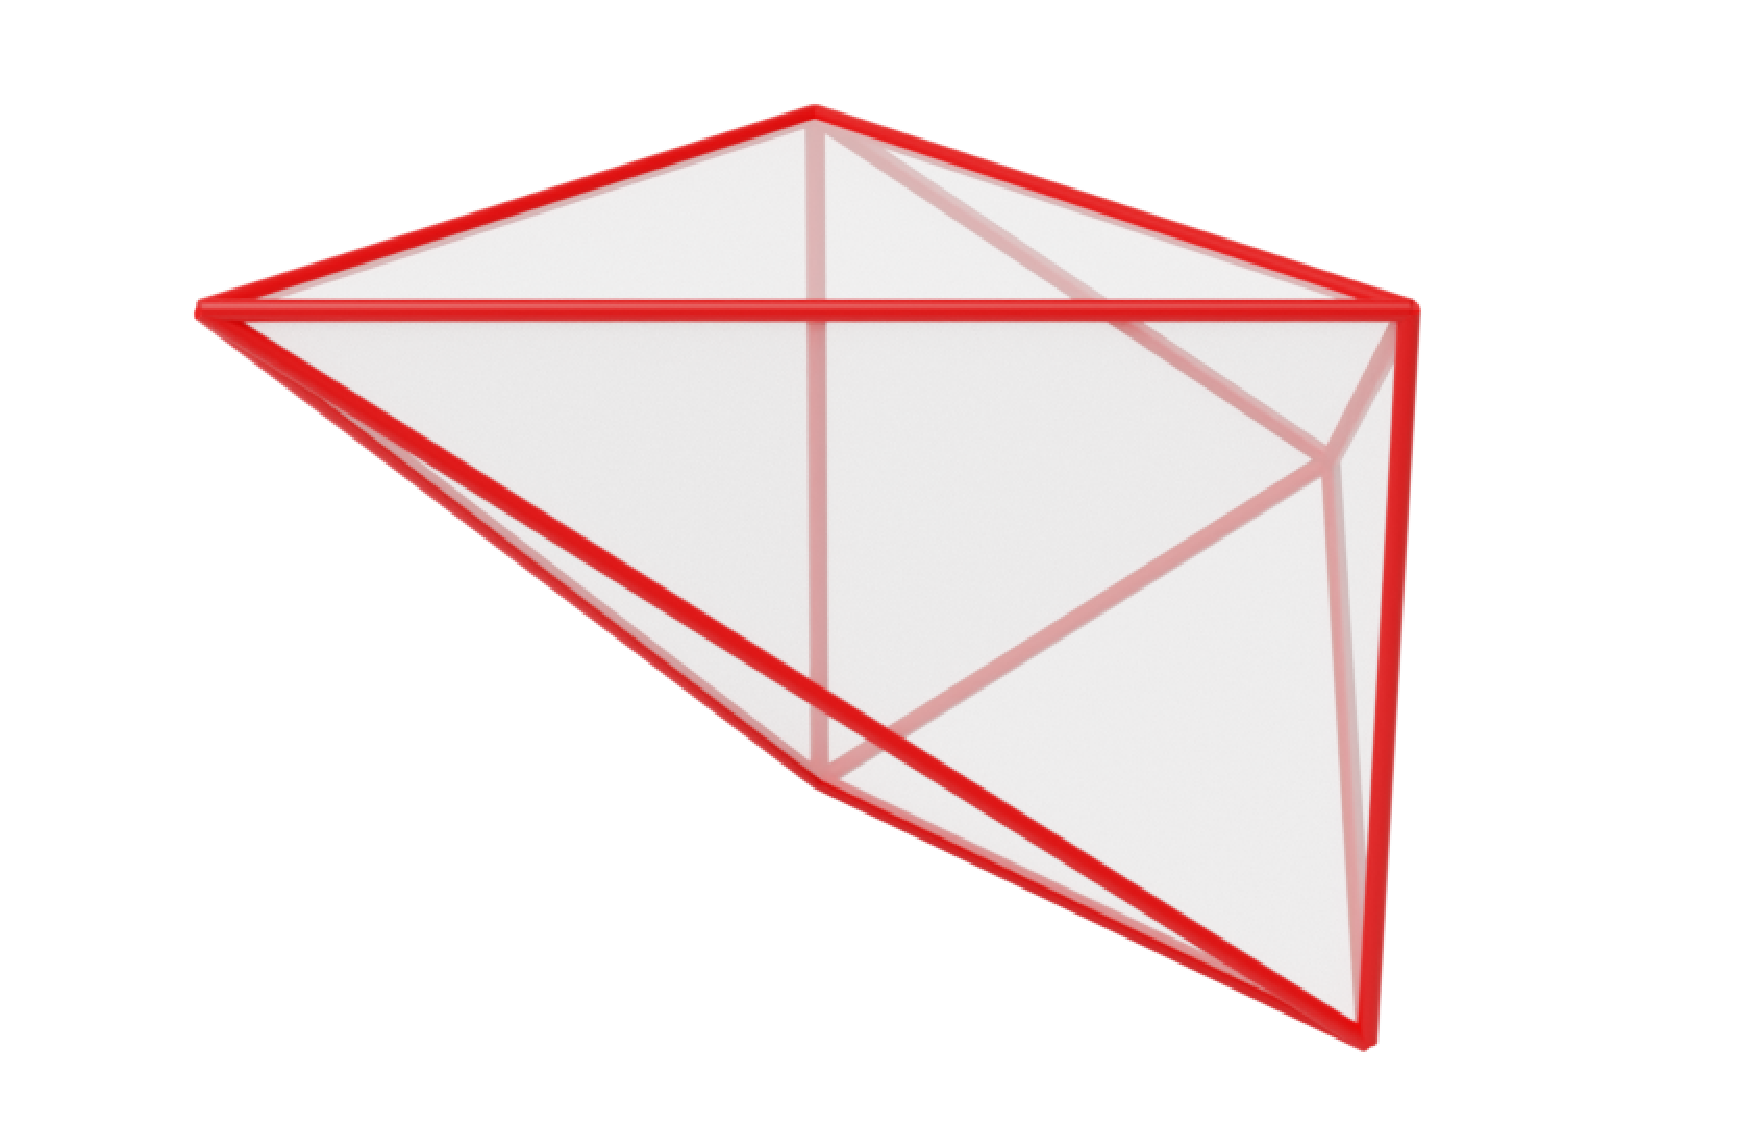
\includegraphics[height=4cm]{images/constrained_diffusion/hull.pdf}
% 		\caption{The convex polytope constraining the diagonals of the triangles for the given bond lengths in the illustrated molecule.
% 			The total design space is the product of this polytope with the 4D flat torus.
% 		}
% 		\label{fig:6s_random_walk_main}
% 	\end{subfigure}
% 	\caption{Illustrations of the parametrisation used to model distribution of polypeptide backbone conformations under anchor point distance constraints as the product of a convex polytope \(\mathbb{P}\) and torus \(\mathbb{T}\): \(\mathbb{P}^{3} \times \mathbb{T}^{4}\).}
% 	\label{fig:han_and_rudolph_main}
% \end{figure}

% Modelling the conformational ensembles of proteins is an important task in the field of molecular biology, particularly in the context of bioengineering and drug discovery.
% In many data-scarce practical settings such as antibody or enzyme design, it is often unnecessary or even undesirable to model the structure of an entire protein, as researchers are primarily interested in specific functional sites with distinct biochemical properties.
% However, generating conformational ensembles for such substructural elements necessitates positional constraints on their endpoints to ensure that they can be accommodated by the remaining scaffold.

% This problem can be reformulated as modelling a spatial chain with spherical joints and fixed end points.
% Following the framework outlined in \textcite{han2006inverse}, we parametrise the conformations of such chains with \(d\) fixed-length links and arbitrary end-point constraints as the product of a convex polytope \(\mathbb{P}\) and torus \(\mathbb{T}\): \(\mathbb{P}^{(d-2)} \times \mathbb{T}^{(d-1)}\).
% The essential idea in this parameterisation is to fix one end point as an ``anchor'' and model the chain as the series of triangles formed by the anchor and each pair of adjacent joints in the chain.
% A point in the polytope corresponds to the lengths of the diagonals of these triangles, and a point in the torus to the angles between each subsequent triangle.
% See~\cref{fig:han_and_rudolph_main} for an illustration and \cref{sec:protein_param} for a full description.
% Using this framework, we model the conformational landscape of the cyclic peptide \textsc{c-AAGAGG}, consisting of a circular polypeptide chain with coinciding endpoints.
% We generate \(10^6\) backbone conformations using tools from molecular dynamics \parencite{eastman2017openmm, hornak2006comparison} and divide them into training and evaluation datasets, (see~\cref{sec:protein_data} for full experimental details).
% Drawing on the definition above, the space on which we effectively parameterise our constrained diffusion models for a circular polypeptide chain of length \(d=6\) is given by the product manifold \(\mathbb{P}^3 \times \mathbb{T}^4\).

To learn a distribution over this space, we leverage the methodology introduced in \cref{sec:bsgm,sec:rbm} for the polytope component \(\mathbb{P}^3\) and \cref{cpt:riemannian_score_based_models} for the torus component \(\mathbb{T}^4\).

A qualitative comparison of samples from the data distribution, our log-barrier and reflected diffusion models, and the uniform distribution is presented in \cref{fig:loop_plot}.
For enhanced visual clarity, we project the modelled spatial chain onto the 2D plane by removing the (unconstrained) torus component of the product manifold and only plotting the planar chains encoded by the (constrained) polytope component (a correlation plot of the full product manifold is presented in \cref{fig:loops_pairs}).

It is immediately obvious that the data distribution is highly multimodal, encompassing a large number of locally optimal conformational clusters.
Nevertheless, both our reflected and log-barrier diffusion models are able to robustly approximate this challenging energetic landscape, producing samples that reflect key conformational states and yielding similar \textsc{MMD} metrics of \(0.032_{\pm{0.021}}\) and \(0.032_{\pm{0.001}}\), respectively.
As a point of comparison, the uniform distribution on the polytope-torus product has an \textsc{MMD} of \(0.112_{\pm{0.001}}\).
The improved relative performance of the log-barrier method seems likely due to the fact that the data for this experiment is largely in the interior of the constrained set, not close to the boundary.

\begin{figure}[tb]
	\centering
	\begin{subfigure}{0.23\textwidth}
		\centering
		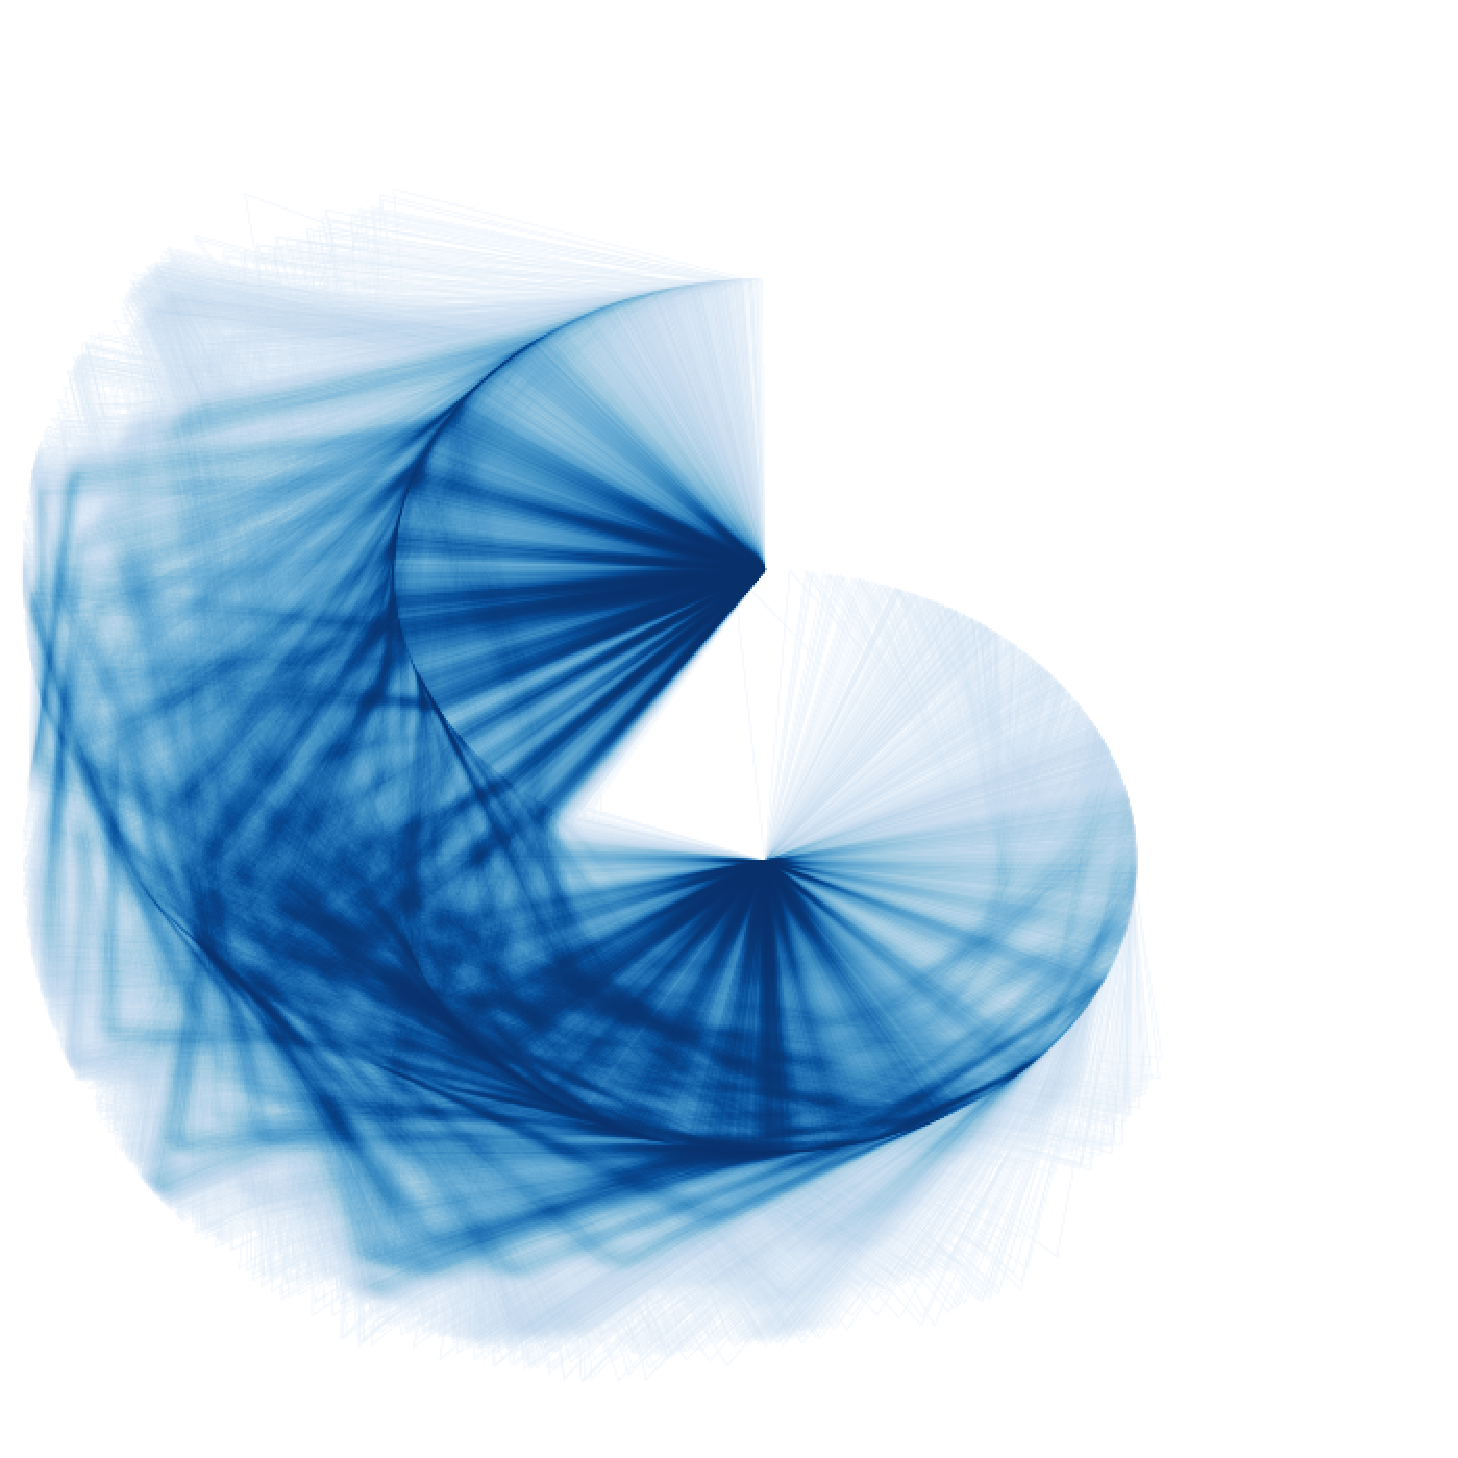
\includegraphics[width=\linewidth]{images/constrained_diffusion/loop_data_dist_2d.pdf}
		\caption{Samples from the data distribution.}
		\label{fig:loop_plot_smoothened}
	\end{subfigure}
	\hfill
	\begin{subfigure}{0.23\textwidth}
		\centering
		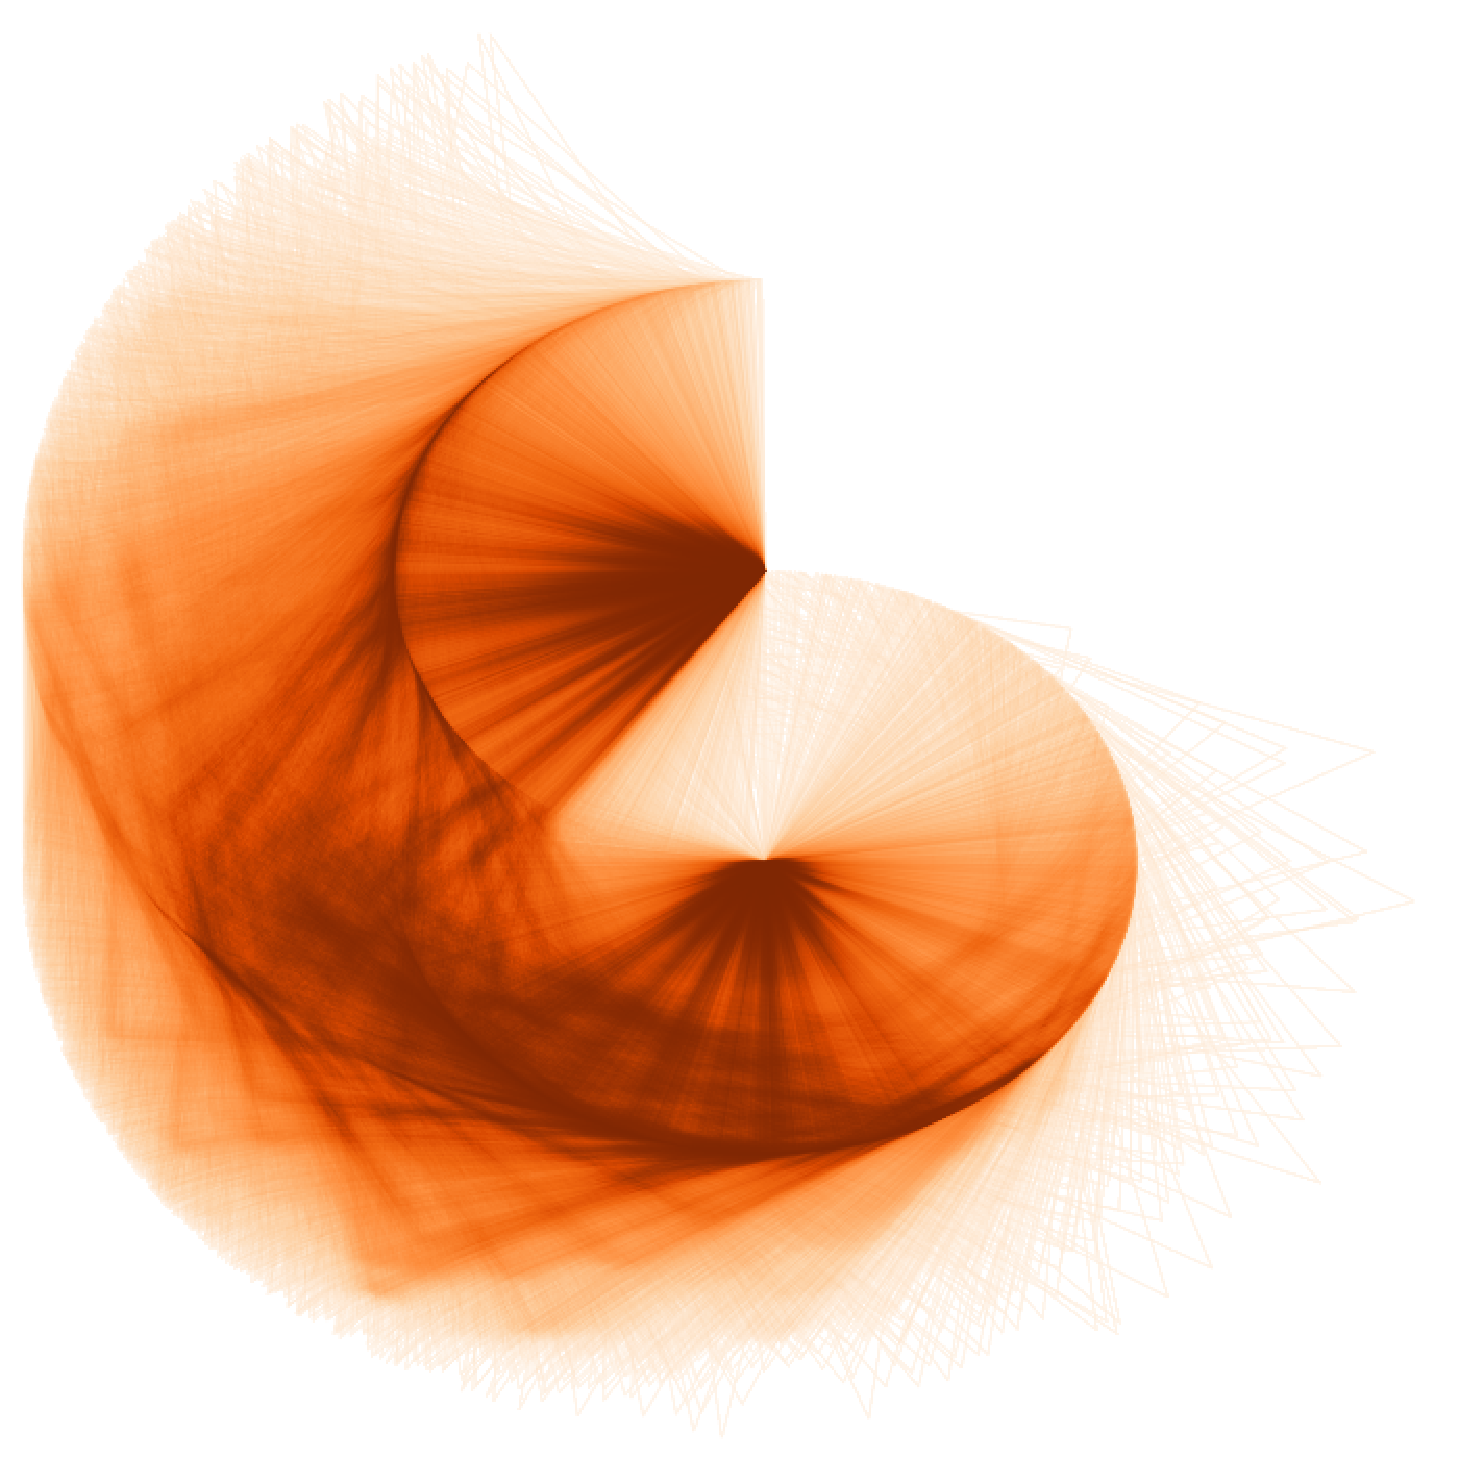
\includegraphics[width=\linewidth]{images/constrained_diffusion/loop_logbarrier_dist_2d.pdf}
		\caption{Samples from our log-barrier diffusion model.}
		\label{fig:loop_plot_logbarrier}
	\end{subfigure}
	\hfill
	\begin{subfigure}{0.23\textwidth}
		\centering
		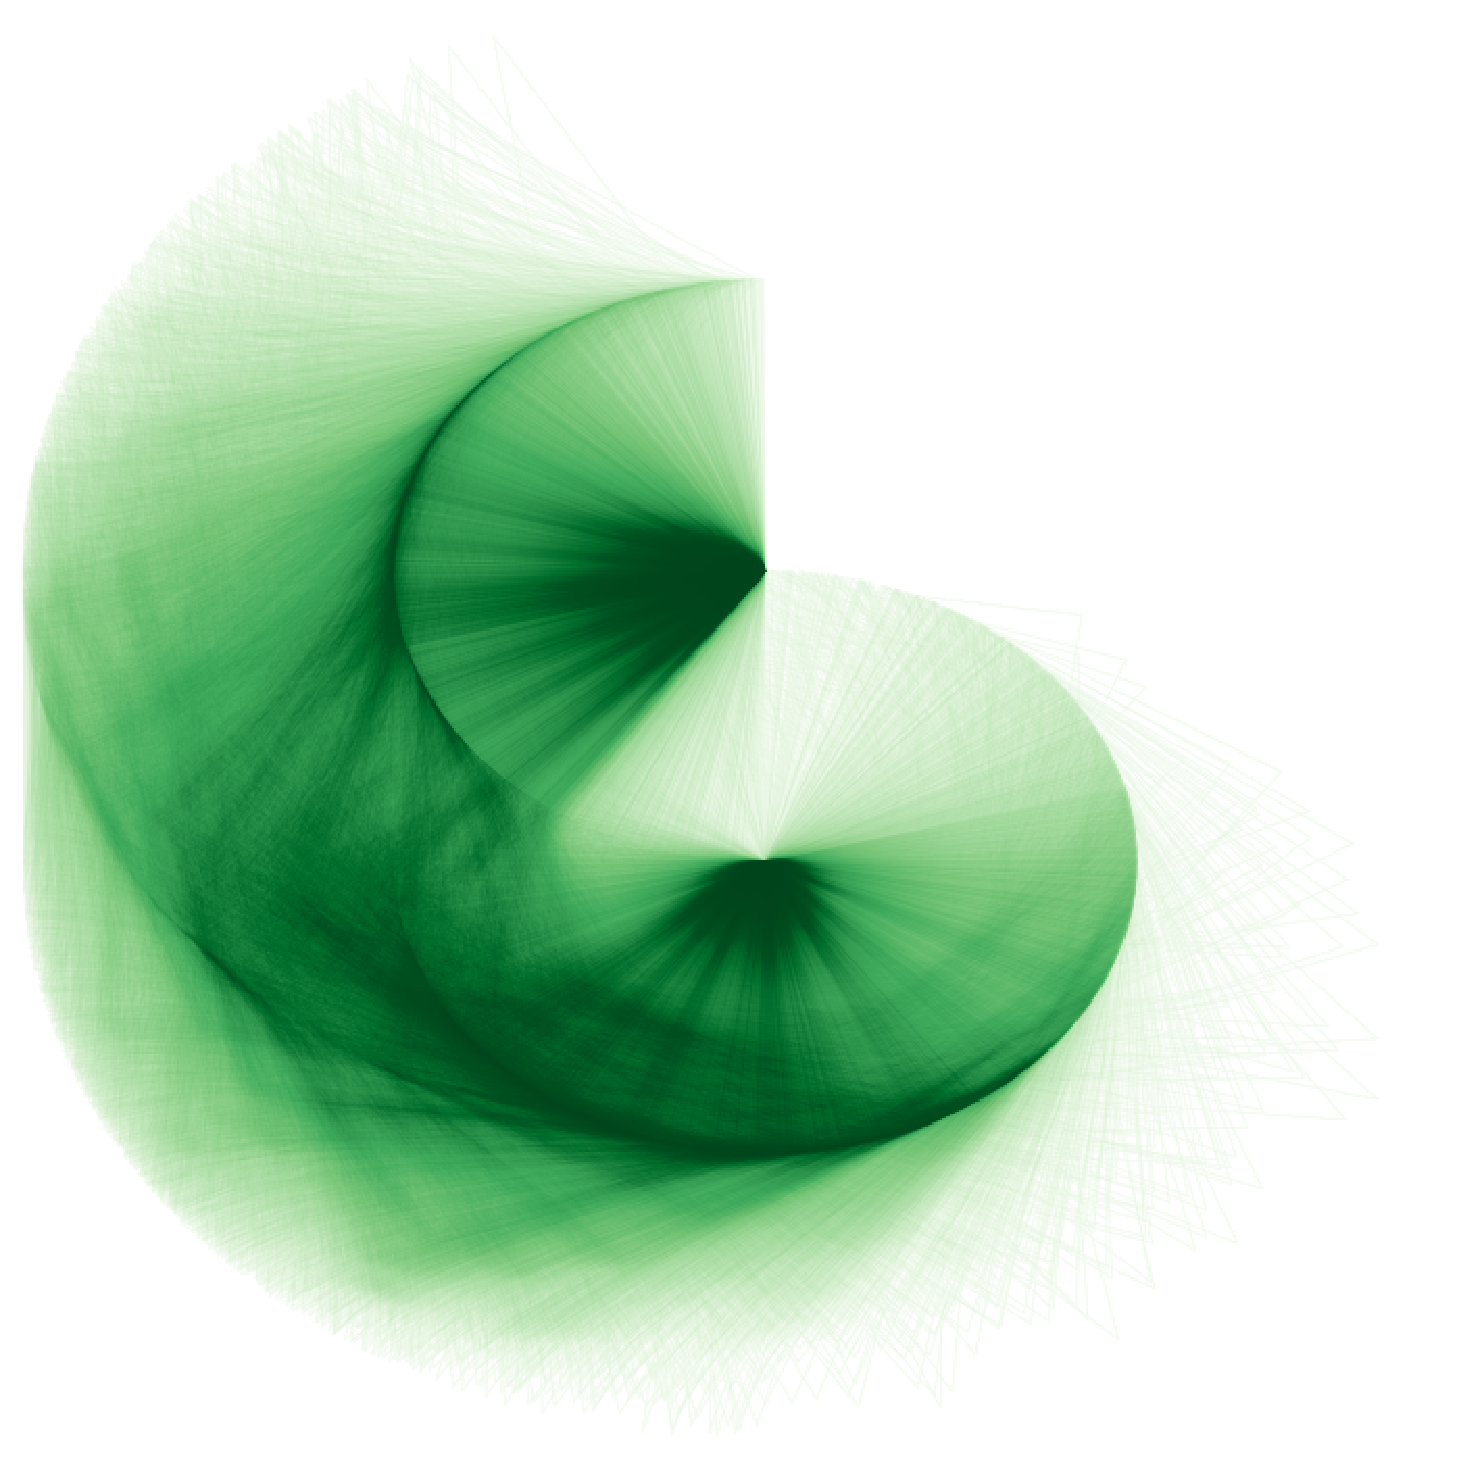
\includegraphics[width=\linewidth]{images/constrained_diffusion/loop_reflected_dist_2d.pdf}
		\caption{Samples from our reflected diffusion model.}
		\label{fig:loop_plot_sampled}
	\end{subfigure}
	\hfill
	\begin{subfigure}{0.23\textwidth}
		\centering
		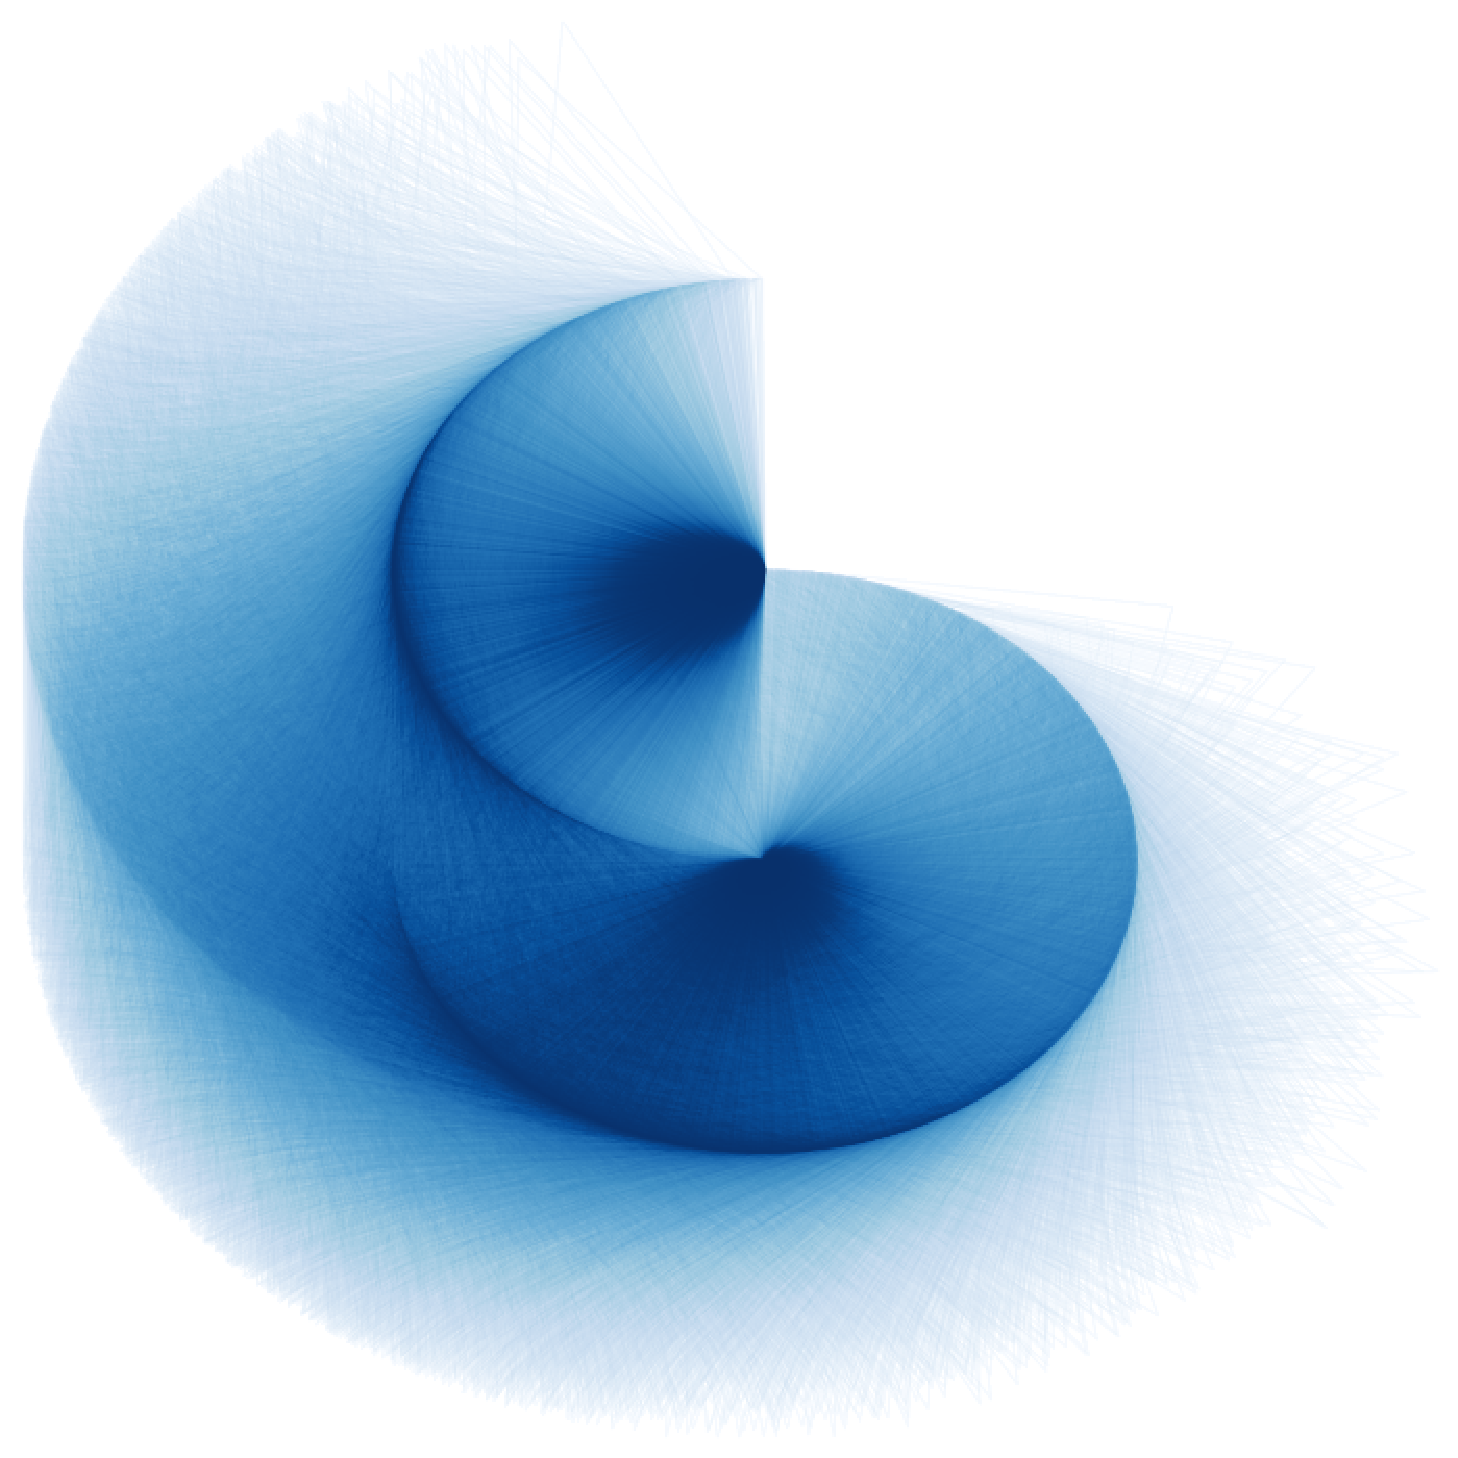
\includegraphics[width=\linewidth]{images/constrained_diffusion/loop_uniform_dist_2d.pdf}
		\caption{Samples from the uniform distribution.}
		\label{fig:loop_plot_uniform}
	\end{subfigure}
	\caption{Planar projection of the modelled \(C_\alpha\) chains from (a) the training dataset, (b) our log-barrier diffusion model, (c) our reflected diffusion model and (d) the uniform distribution.
		Additional results and full correlation plots are postponed to~\cref{sec:app_protein_exp}.
	}
	\label{fig:loop_plot}
\end{figure}

\section{Conclusion}

Learning complex distributions supported on constrained spaces is a crucial task in many natural and engineering sciences, including computational statistics \parencite{Morris2002}, robotics \parencite{han2006inverse}, quantum physics \parencite{lukens2020practical} and computational biology \parencite{Thiele2013}.
In this chapter we extend continuous diffusion models to this setting, proposing two complementary approaches---one based on log-barrier methods and the other on the reflected Brownian motion.
For both approaches, we derive the time-reversal formula, propose discretisation schemes and extend the score-matching toolbox.
We demonstrated the utility of our methods on a range of synthetic and real-world tasks.
This including the constrained conformational modelling of proteins and robotic arms, and find that reflected methods, while enjoying fewer theoretical guarantees than their log-barrier counterparts, often yield preferable results.

We conclude by highlighting important future directions.
First, the computational cost of performing the reflection when discretising the reflected Brownian motion is high.
Finding numerically efficient approximations of the reflected process is therefore necessary to extend this methodology to high dimension settings.
Second, the retraction used in place of the exponential map for the barrier method leads to a high number of discretisation steps to ensure a good approximation.
Designing a faster forward process for the log-barrier method is key to targeting more complex distributions.


